\documentclass[a4paper,11pt,fleqn,twoside,openright]{memoir} 	% Openright aabner kapitler paa hoejresider (openany begge)

%%%% PACKAGES %%%%

% ¤¤ Oversaettelse og tegnsaetning ¤¤ %
\usepackage[utf8]{inputenc}					% Input-indkodning af tegnsaet (UTF8)
\usepackage[english]{babel}					% Dokumentets sprog
\usepackage[T1]{fontenc}					% Output-indkodning af tegnsaet (T1)
\usepackage{ragged2e,anyfontsize}			% Justering af elementer
\usepackage{fixltx2e}						% Retter forskellige fejl i LaTeX-kernen
																			
% ¤¤ Figurer og tabeller (floats) ¤¤ %
\usepackage{graphicx} 						% Haandtering af eksterne billeder (JPG, PNG, PDF)
\usepackage{multirow}                		% Fletning af raekker og kolonner (\multicolumn og \multirow)
\usepackage{colortbl} 						% Farver i tabeller (fx \columncolor, \rowcolor og \cellcolor)
\usepackage[dvipsnames]{xcolor}				% Definer farver med \definecolor. Se mere: http://en.wikibooks.org/wiki/LaTeX/Colors
\usepackage{flafter}						% Soerger for at floats ikke optraeder i teksten foer deres reference
\let\newfloat\relax 						% Justering mellem float-pakken og memoir
\usepackage{float}							% Muliggoer eksakt placering af floats, f.eks. \begin{figure}[H]
%\usepackage{eso-pic}						% Tilfoej billedekommandoer paa hver side
%\usepackage{wrapfig}						% Indsaettelse af figurer omsvoebt af tekst. \begin{wrapfigure}{Placering}{Stoerrelse}
%\usepackage{multicol}         	        	% Muliggoer tekst i spalter
%\usepackage{rotating}						% Rotation af tekst med \begin{sideways}...\end{sideways}
\usepackage{array}


% ¤¤ Matematik mm. ¤¤
\usepackage{amsmath,amssymb,stmaryrd} 		% Avancerede matematik-udvidelser
\usepackage{mathtools}						% Andre matematik- og tegnudvidelser
\usepackage{textcomp}                 		% Symbol-udvidelser (f.eks. promille-tegn med \textperthousand )
\usepackage{siunitx}						% Flot og konsistent praesentation af tal og enheder med \si{enhed} og \SI{tal}{enhed}
\sisetup{output-decimal-marker = {,}}		% Opsaetning af \SI (DE for komma som decimalseparator) 
\usepackage[version=3]{mhchem} 				% Kemi-pakke til flot og let notation af formler, f.eks. \ce{Fe2O3}
%\usepackage{rsphrase}						% Kemi-pakke til RS-saetninger, f.eks. \rsphrase{R1}

% ¤¤ Referencer og kilder ¤¤ %
\usepackage[danish]{varioref}				% Muliggoer bl.a. krydshenvisninger med sidetal (\vref)
\usepackage{natbib}							% Udvidelse med naturvidenskabelige citationsmodeller
%\usepackage{xr}							% Referencer til eksternt dokument med \externaldocument{<NAVN>}
%\usepackage{glossaries}					% Terminologi- eller symbolliste (se mere i Daleifs Latex-bog)

% Quotation %
\usepackage{csquotes}

% ¤¤ Misc. ¤¤ %
\usepackage{listings}						% Placer kildekode i dokumentet med \begin{lstlisting}...\end{lstlisting}
\usepackage{lipsum}							% Dummy text \lipsum[..]
\usepackage[shortlabels]{enumitem}			% Muliggoer enkelt konfiguration af lister
\usepackage{pdfpages}						% Goer det muligt at inkludere pdf-dokumenter med kommandoen \includepdf[pages={x-y}]{fil.pdf}	
\pdfoptionpdfminorversion=6					% Muliggoer inkludering af pdf dokumenter, af version 1.6 og hoejere
\pretolerance=2500 							% Justering af afstand mellem ord (hoejt tal, mindre orddeling og mere luft mellem ord)

% Kommentarer og rettelser med \fxnote. Med 'final' i stedet for 'draft' udloeser hver note en error i den faerdige rapport.
\usepackage[footnote,draft,danish,silent,nomargin]{fixme}		

\usepackage{todonotes}

\usepackage{lastpage}

%%%% CUSTOM SETTINGS %%%%

% ¤¤ Marginer ¤¤ %
\setlrmarginsandblock{3.5cm}{2.5cm}{*}		% \setlrmarginsandblock{Indbinding}{Kant}{Ratio}
\setulmarginsandblock{2.5cm}{3.0cm}{*}		% \setulmarginsandblock{Top}{Bund}{Ratio}
\checkandfixthelayout 						% Oversaetter vaerdier til brug for andre pakker

%	¤¤ Afsnitsformatering ¤¤ %
\setlength{\parindent}{0mm}           		% Stoerrelse af indryk
\setlength{\parskip}{3mm}          			% Afstand mellem afsnit ved brug af double Enter
\linespread{1,1}							% Linie afstand

%Definition bokses %
\usepackage{xcolor}
\usepackage{ntheorem}
\usepackage{mdframed}

\theoremstyle{break}
\theoremheaderfont{\bfseries}
\newmdtheoremenv[%
linecolor=gray,leftmargin=60,%
rightmargin=40,
backgroundcolor=gray!40,%
innertopmargin=8pt,%
ntheorem]{defi}{Definition}[section]

% ¤¤ Litteraturlisten ¤¤ %
\bibpunct[,]{[}{]}{;}{a}{,}{,} 				% Definerer de 6 parametre ved Harvard henvisning (bl.a. parantestype og seperatortegn)
\bibliographystyle{bibtex/harvard}			% Udseende af litteraturlisten.

% ¤¤ Indholdsfortegnelse ¤¤ %
\setsecnumdepth{subsection}		 			% Dybden af nummerede overkrifter (part/chapter/section/subsection)
\maxsecnumdepth{subsection}					% Dokumentklassens graense for nummereringsdybde
\settocdepth{subsection} 					% Dybden af indholdsfortegnelsen

% ¤¤ Lister ¤¤ %
\setlist{
  topsep=0pt,								% Vertikal afstand mellem tekst og listen
  itemsep=-1ex,								% Vertikal afstand mellem items
} 

% ¤¤ Visuelle referencer ¤¤ %
\usepackage[colorlinks]{hyperref}			% Danner klikbare referencer (hyperlinks) i dokumentet.
\hypersetup{colorlinks = true,				% Opsaetning af farvede hyperlinks (interne links, citeringer og URL)
    linkcolor = black,
    citecolor = black,
    urlcolor = black
}

% ¤¤ Opsaetning af figur- og tabeltekst ¤¤ %
\captionnamefont{\small\bfseries\itshape}	% Opsaetning af tekstdelen ('Figur' eller 'Tabel')
\captiontitlefont{\small}					% Opsaetning af nummerering
\captiondelim{. }							% Seperator mellem nummerering og figurtekst
\hangcaption								% Venstrejusterer flere-liniers figurtekst under hinanden
\captionwidth{\linewidth}					% Bredden af figurteksten
\setlength{\belowcaptionskip}{0pt}			% Afstand under figurteksten
		
% ¤¤ Opsaetning af listings ¤¤ %
\definecolor{commentGreen}{RGB}{34,139,24}
\definecolor{stringPurple}{RGB}{208,76,239}

\lstset{
  numbers=left,
  stepnumber=1,    
  firstnumber=1,
  numberfirstline=true
}

\usepackage{xcolor}

\lstdefinestyle{MyLang}{
    basicstyle=\small\ttfamily\color{magenta},%
    breaklines=true,%                                      allow line breaks
    moredelim=[s][\color{green!50!black}\ttfamily]{'}{'},% single quotes in green
    moredelim=*[s][\color{black}\ttfamily]{options}{\}},%  options in black (until trailing })
    commentstyle={\color{gray}\itshape},%                  gray italics for comments
    morecomment=[l]{//},%                                  define // comment
    emph={%
        %                                            literal strings listed here
        },emphstyle={\color{blue}\ttfamily},%              and formatted in blue
    alsoletter={:,|,;},%
    morekeywords={:,|,;},%                                 define the special characters
    keywordstyle={\color{black}},%                         and format them in black  
}	
\lstset{language=Matlab,					% Sprog
	basicstyle=\ttfamily\scriptsize,		% Opsaetning af teksten
	%keywords={for,if,while,else,elseif,		% Noegleord at fremhaeve
	%		  end,break,return,case,
	%		  switch,function},
	keywordstyle=\color{blue},				% Opsaetning af noegleord
	commentstyle=\color{commentGreen},		% Opsaetning af kommentarer
	stringstyle=\color{stringPurple},		% Opsaetning af strenge
	showstringspaces=false,					% Mellemrum i strenge enten vist eller blanke
	%numbers=left, numberstyle=\tiny,		% Linjenumre
	extendedchars=true, 					% Tillader specielle karakterer
	columns=flexible,						% Kolonnejustering
	breaklines, breakatwhitespace=true,		% Bryd lange linjer
}



% ¤¤ Navngivning ¤¤ %
%\addto\captionsdanish{
%	\renewcommand\appendixname{Appendiks}
%	\renewcommand\contentsname{Indholdsfortegnelse}	
%	\renewcommand\appendixpagename{Appendiks}
%	\renewcommand\appendixtocname{Appendiks}
%	\renewcommand\cftchaptername{\chaptername~}				% Skriver "Kapitel" foran kapitlerne i indholdsfortegnelsen
%	\renewcommand\cftappendixname{\appendixname~}			% Skriver "Appendiks" foran appendiks i indholdsfortegnelsen
%	}

% ¤¤ Kapiteludssende ¤¤ %
\definecolor{numbercolor}{gray}{0.7}		% Definerer en farve til brug til kapiteludseende
\newif\ifchapternonum

\makechapterstyle{jenor}{					% Definerer kapiteludseende frem til ...
  \renewcommand\beforechapskip{0pt}
  \renewcommand\printchaptername{}
  \renewcommand\printchapternum{}
  \renewcommand\printchapternonum{\chapternonumtrue}
  \renewcommand\chaptitlefont{\fontfamily{pbk}\fontseries{db}\fontshape{n}\fontsize{25}{35}\selectfont\raggedleft}
  \renewcommand\chapnumfont{\fontfamily{pbk}\fontseries{m}\fontshape{n}\fontsize{1in}{0in}\selectfont\color{numbercolor}}
  \renewcommand\printchaptertitle[1]{%
    \noindent
    \ifchapternonum
    \begin{tabularx}{\textwidth}{X}
    {\let\\\newline\chaptitlefont ##1\par} 
    \end{tabularx}
    \par\vskip-2.5mm\hrule
    \else
    \begin{tabularx}{\textwidth}{Xl}
    {\parbox[b]{\linewidth}{\chaptitlefont ##1}} & \raisebox{-15pt}{\chapnumfont \thechapter}
    \end{tabularx}
    \par\vskip2mm\hrule
    \fi
  }
}											% ... her

\chapterstyle{jenor}						% Valg af kapiteludseende - Google 'memoir chapter styles' for alternativer

% ¤¤ Sidehoved ¤¤ %

\makepagestyle{Uni}							% Definerer sidehoved og sidefod udseende frem til ...
\makepsmarks{Uni}{%
	\createmark{chapter}{left}{shownumber}{}{. \ }
	\createmark{section}{right}{shownumber}{}{. \ }
	\createplainmark{toc}{both}{\contentsname}
	\createplainmark{lof}{both}{\listfigurename}
	\createplainmark{lot}{both}{\listtablename}
	\createplainmark{bib}{both}{\bibname}
	\createplainmark{index}{both}{\indexname}
	\createplainmark{glossary}{both}{\glossaryname}
}
\nouppercaseheads											% Ingen Caps oenskes

\makeevenhead{Uni}{Group SW408F16}{}{\leftmark}				% Definerer lige siders sidehoved (\makeevenhead{Navn}{Venstre}{Center}{Hoejre})
\makeoddhead{Uni}{\rightmark}{}{Aalborg University}			% Definerer ulige siders sidehoved (\makeoddhead{Navn}{Venstre}{Center}{Hoejre})
\makeevenfoot{Uni}{\thepage}{}{}							% Definerer lige siders sidefod (\makeevenfoot{Navn}{Venstre}{Center}{Hoejre})
\makeoddfoot{Uni}{}{}{\thepage}								% Definerer ulige siders sidefod (\makeoddfoot{Navn}{Venstre}{Center}{Hoejre})
\makeheadrule{Uni}{\textwidth}{0.5pt}						% Tilfoejer en streg under sidehovedets indhold
\makefootrule{Uni}{\textwidth}{0.5pt}{1mm}					% Tilfoejer en streg under sidefodens indhold

\copypagestyle{Unichap}{Uni}								% Sidehoved for kapitelsider defineres som standardsider, men med blank sidehoved
\makeoddhead{Unichap}{}{}{}
\makeevenhead{Unichap}{}{}{}
\makeheadrule{Unichap}{\textwidth}{0pt}
\aliaspagestyle{chapter}{Unichap}							% Den ny style vaelges til at gaelde for chapters
															% ... her
															
\pagestyle{Uni}												% Valg af sidehoved og sidefod (benyt "plain" for ingen sidehoved/fod)


%%%% CUSTOM COMMANDS %%%%

% ¤¤ Billede hack ¤¤ %										% Indsaet figurer nemt med \figur{Stoerrelse}{Fil}{Figurtekst}{Label}
\newcommand{\figur}[4]{
		\begin{figure}[H] \centering
			\includegraphics[width=#1\textwidth]{billeder/#2}
			\caption{#3}\label{#4}
		\end{figure} 
}

\newcommand\tab[1][1cm]{\hspace*{#1}}

% ¤¤ Specielle tegn ¤¤ %
\newcommand{\decC}{^{\circ}\text{C}}
\newcommand{\dec}{^{\circ}}
\newcommand{\m}{\cdot}


%%%% ORDDELING %%%%

\hyphenation{}											% Preamble indlaeses
\raggedbottom													% Soerger for at LaTeX ikke "straekker" teksten

%\includeonly{file1,file2}										% Inkluder kun specifikke filer (kommasepareret liste)

\begin{document}												% Starter dokumentet - obligatorisk


\frontmatter													% Forindhold - nummereres med romertal

	\thispagestyle{empty}
\begin{flushright}
\vspace{3cm}

\phantom{hul}

\phantom{hul}

\phantom{hul}

\textsl{\Huge Dumpsty} \\ \vspace{1cm}

\rule{13cm}{3mm} \\ \vspace{1.5cm}
\vspace{1cm}

%\includegraphics[width=0.9\textwidth]{}


\vspace{7cm} 
\textsc{\Large P5 Project \\
Group SW510E16 \\
Software\\
Aalborg University\\
21st Dec 2016\\}
\end{flushright}

\cleardoublepage												% Indsaetter tom side, saa naeste kapitel starter paa hoejre side (hvis noedvendigt)
% Dette er LaTeX-versionen af titelbladet for TNB studenterrapporter
% Filen kræver:
% Universitetets logo:  AAU-logo-stud-UK eller AAU-logo-stud-DK
% Synopsis: En fil ved navn synopsis.tex

% Udarbejdet af: Jesper Nørgaard (jesper@noergaard.eu) 10. april 2012

\phantomsection
\pdfbookmark[0]{Titelblad}{titelblad}
\thispagestyle{empty}

\begin{minipage}[t]{0.48\textwidth}
\vspace*{-25pt}			%\vspace*{-9pt}

\includegraphics[height=4cm]{billeder/AAU-logo-stud-UK-RGB}
\end{minipage}
\hfill
\begin{minipage}[t]{0.48\textwidth}
{\small 
\textbf{Fourth semester at}\\
\textbf{Department of Computer Science}  \\
Software \\
Selma Lagerlöfs Vej 300 \\
9220 Aalborg East, DK \\
http://www.cs.aau.dk/}
\end{minipage}

\vspace*{1cm}

\begin{minipage}[t]{0.48\textwidth}
\textbf{Title:} \\[5pt]\bigskip\hspace{2ex}
Dumpsty

\textbf{Project:} \\[5pt]\bigskip\hspace{2ex}
P5-project

\textbf{Project period:} \\[5pt]\bigskip\hspace{2ex}
September 2016 - December 2016

\textbf{Project group:} \\[5pt]\bigskip\hspace{2ex}
SW510E16	

\textbf{Participants:} \\[5pt]\hspace*{2ex}
Christian Dannesboe \\\hspace*{2ex}
Frederik Børsting Lund \\\hspace*{2ex}
Karrar Al-Sami \\\hspace*{2ex}
Mark Kloch Haurum \\\hspace*{2ex}
Lasse Lyngø Nielsen \\\hspace*{2ex}
Søren Lyng \\\hspace*{2ex}

\textbf{Supervisor:} \\[5pt]\hspace*{2ex}
Bent Thomsen

\vspace*{1cm}


\textbf{Pagecount: \pageref{LastPage}} \\
\textbf{Appendix range: 26} \\ 
\textbf{Published 21-12-2016}

\end{minipage}
\hfill
\begin{minipage}[t]{0.483\textwidth}
Synopsis: \\[5pt]
\fbox{\parbox{7cm}{\bigskipThis project is about the design and implementation of a trash bin which is to catch the trash thrown at it. This is done using a Arduino Mega 2560 for the trash bin and a Microsoft Kinect for detecting and tracking the thrown trash. 
\newline

The report covers the analysis of the problem and hardware, a design specification, system design and implementation. The system is then tested and the results are discussed and concluded upon. 
\newline



\bigskip}}
\end{minipage}

\vfill

{\footnotesize\itshape The content of the article is freely available, but may only be published with reference to the article.}

% Rapportens indhold er frit tilgængeligt, men offentliggørelse (med kildeangivelse) må kun ske efter aftale med forfatterne.
% The content of the report is freely available, but publication (with source reference) may only take place in agreement with the authors.

\cleardoublepage
\chapter*{Preface}
This report is part of the fifth semester project made by project group SW510E16 at Aalborg University, Software Engineering starting from the 2nd of September to the 21st of December 2016. \newline
The project is based on the \textit{Aalborg-model} study method, where problem and project based learning is the focus. The theme of this semester is to make an embedded system with real-time constraints. The project group chose to make a trash bin that should be able to catch the trash thrown at it. \newline

The project group would like to thank the project supervisor Bent Thomsen, for his  support and help throughout the project. 
\newline
\newline
\newline
\newline


{\Huge\textbf{Signatures}}
\newline
\newline


\begin{table}[H]
	\centering
	\begin{tabular}{c c c}
		\underline{\phantom{mmmmmmmmmmmmmm}} & \underline{\phantom{mmmmmmmmmmmmmm}} & \underline{\phantom{mmmmmmmmmmmmmm}} \\
		Christian Dannesboe			& Frederik Børsting Lund 		& Karrar Al-Sami 			\\
		&&\\
		&&\\
		\underline{\phantom{mmmmmmmmmmmmmm}} & \underline{\phantom{mmmmmmmmmmmmmm}} & \underline{\phantom{mmmmmmmmmmmmmm}} \\
		Mark Kloch Haurum			& Lasse Lyngø Nielsen 		& Søren Lyng 				\\
		&&\\
		&&\\
		
	\end{tabular}
\end{table}


\chapter*{Reading guide}
Throughout the report sources are referred to by the Harvard citation method. When a source is listed in the report, the last name of the author and a publication year is listed. The sources are all listed alphabetically in the \textit{\textbf{Bibliography}} chapter. \newline
\textit{This is an example of a source listed in the report: \textbf{\citep{safe}}.} \newline
The source may refer to either the whole section or to only that sentence. The way this differs depends on the placement of the dot. If the dot is after the source, then that source refers to the sentence and if the dot is before the source, then the source refers to the whole section. 


When referring to figures, tables and source code, numbers are used. Depending on which chapter and number of figure/table, the number is defined. \newline
\textit{This example can be used: In chapter X we want to refer to the second figure. This is done by giving the figure number \textbf{X.2}, where X is the number of the chapter we're referring to.}
\newline


When referring to source code, we're using code snippets. These code snippets aren't necessarily the full source code, but may be shorter version of it and/or missing comments. When code has been removed in the snippets, the use of three dots are used:  \textit\textbf{{"..."}}, these dots show that some code altering has been made in the snippet, whether it's because it's long and irrelevant for understanding the purpose of the code, or because we're simply just trying to explain those few lines. 


Throughout the report requirements are split into four colours with four different meanings. The colour blue refers to new requirements or focus requirements for that specific increment. The colour green refers to a requirement being fulfilled. Orange means that the requirement is fulfilled but has been changed. Red means that the requirement has been changed, but not yet fulfilled. 

\cleardoublepage

%%%% Indholdsfortegnelse (TOC) %%%%

\phantomsection													% Kunstigt afsnit, som hyperlinks kan 'holde fast i'
\pdfbookmark[0]{Indholdsfortegnelse}{indhold}					% Tildeler en klikbar bookmark til den endelige PDF
\tableofcontents*												% Indholdsfortegnelsen (kaldet ToC) 
\addcontentsline{toc}{chapter}{\listfigurename}
\addcontentsline{toc}{chapter}{\lstlistlistingname}
%\addtocontents{toc}{\protect\newpage}							% Fremtvinger sideskift i ToC hvis noedvendig (der hvor koden placeres)
\newpage
\listoffigures*
\newpage
\lstlistoflistings
\mainmatter														% Hovedindhold - nummereres fra side 1

%%%% Rapportindhold %%%% 										% Rapportindholdet boer IKKE indeholde broedtekst - KUN includede filer!

%% Indledende %%												% Opdel evt. i passende afsnit for overblikkets skyld

 \chapter{Introduction}
\label{chap:Introduction}
An embedded system is a computer system which only has a few functions. It is embedded as a part of a whole device, which then also includes hardware and/or mechanical components. Embedded systems are everywhere in our everyday lives. The range for embedded systems could be all from saving lives with pacemakers to fun gadgets. \citep{es}

An embedded system as a gadget, is a technological and small object or apparatus, which has a certain functionality. This functionality is limited to a certain niche. \newline
In this project, the embedded system in consideration would be designed as a gadget, with the sole purpose of catching trash thrown at it. A trash bin that can catch trash would make the act of cleaning more fun and interactive, and the availability of each individual trash bin would be tremendously increased, because it will be able to move around.

For this gadget to be usable, it must be designed as a real-time system, as this system will have certain deadlines for each task to be executed in time. The trash bin must be able to identify an object coming towards it, make some computation to identify a point to catch it from, and then compute a path to catch the object. All this must be done before the object lands on the ground, which makes the use of real-time system design a part of this project. A real-time system is a software system which is subject to a real-time constraint, and the system must control and affect an environment, by receiving data and process these, within a certain time limit. 





\chapter{Process model}
\label{Process model}
Process models for software development is a representation of the process and the activities required for developing the software. In software engineering there is two different development approaches, pland-driven and agile development. The plan-driven approach is based on sperate development stages and iterations can occur within the activities e.g. the implementation of the software. The agile approach the specification, design, implementation and tests are all iterated on as a whole. \citep{sommerville}

The process model is a meld of elements from both plan driven and agile development. The process is plan driven in so far as to include a clear goal of what the initial requirements of the system are. The process model is very agile in that, although there is a clear outline as to what the requirements are, these are incrementally approached, with a simple starting point becoming increasingly covering of the project vision through the subsequent increments. The reason the group approached this project with our 'own' process model is to better explain what we're actually doing, rather than forcing ourselves into picking a development method and try to explain what we're doing according to that method.

The increments will be split up into four sections. Initially some of the already known requirements will be considered from previous increments and for the first increment from the analysis chapter, and these requirements will be the topic of the increment.
After the initial requirement consideration, a design phase follows which details the design and problem considerations preceding the implementation. The design phase is then followed by an implementation phase which will explain the implementation process. The final phase is an evaluation of the increment and will concern whether the requirements were fulfilled, if an requirement needs to be altered, or if an requirement will be continued in the following increment. The evaluation will also include several tests of the implementation, in order to see what works and what doesn't work. The evaluated requirements from an increment will then become the starting point of the next increment. An illustration of the process model described can be found in figure \ref{pm}.

The process includes both pair programming and pair writing, which is to promote cooperation and attempt to avoid having a single individual involved in a task beyond their capabilities and to get a second opinion. This is also to ensure that information is quickly communicated and exchanged by group members. The process uses pair programming because it promotes better programming and is usually very motivating in socially engaging issues with cooperation of project members.


\begin{figure}[h]
	\centering
	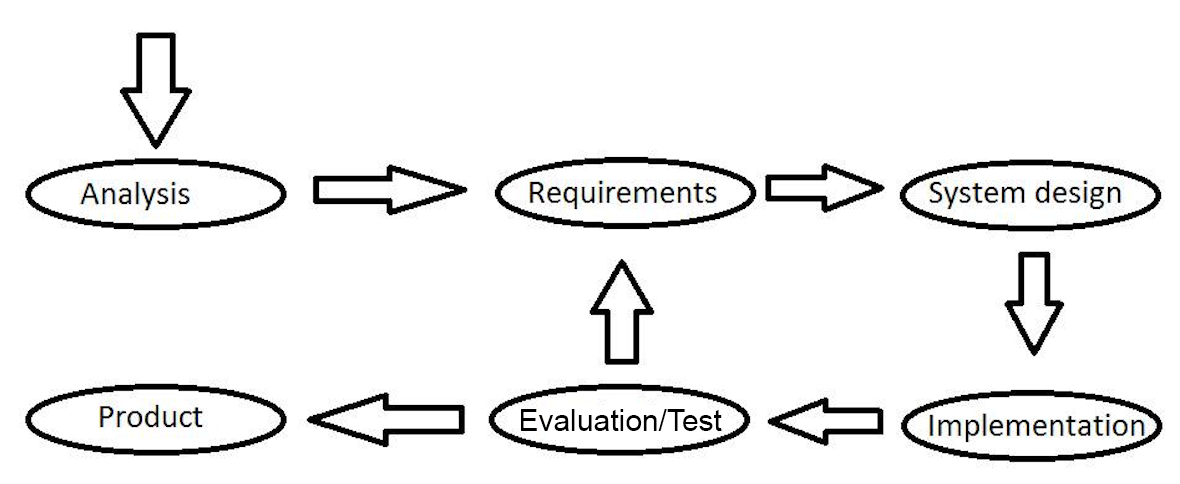
\includegraphics[scale=0.30]{billeder/process-model}
	\caption{Process model used for the project}
	\label{pm}
\end{figure}
\chapter{Toolchain}
The following tools has been used to create the report and the product of the project. Every tool in the toolchain has a description stating the benefits and use of the tool.


\begin{itemize}
	\item GitHub
	\item TeX Studio
	\item Visual Studio
	\item Arduino IDE 1.0.3
	\item BoundT
	\item UPPAAL
	\item ArduinoUnit
\end{itemize}


\section*{Use of tools}
\textbf{GitHub} is used with the intention of merging and sharing documents. This tool is also used here to verify each version of the documentation and code, to ensure that everyone has the latest update of the project.\newline
\textbf{TeX Studio} is used as a writing environment when writing with the markup language LaTeX. After some experience it has proven to be a great tool for creating a report. This tool in concoction with GitHub makes it possible to work on the project in pairs or alone, with little merging conflicts. \newline
\textbf{Visual Studio} is used in this project to create the C\# code for the Kinect. \newline
\textbf{Arduino IDE 1.0.3} is used in this project to code the Arduino. Any later IDE is not suitable for this project, which will be explained in the report. \newline
\textbf{BoundT} is used to calculate the bounds of the code, which will be used in a WCET-analysis. \citep{boundt} \newline
\textbf{UPPAAL} is an integrated tool environment for modeling, validation and verification of real-time system. \citep{uppaal} \newline
\textbf{ArduinoUnit} is a unit test framework for arduino projects and is used for the unit tests in the tests chapter, \ref{chap:Tests}, of this project. \citep{au}



\chapter{Analysis}
\label{chap:Analysis}
From the analysis chapter it should be possible to derive the requirements for the smart trash bin, Dumpsty. The initial user story will help make the user requirements for the project. After the user requirements has been formed, the information from the user story will be analysed in greater detail, depicting three different phases of the process: Throwing, detecting/tracking and catching. These three phases will be the inspiration for the system requirements. 
The analysis chapter will end up with a problem statement for the project. 

\section{User story}
\label{sec:User story}
Benjamin is a software engineer who is tired of wasting his precious time on the job with walking back and forth from the trash bin in his office, and therefore wants to be able to throw his trash in the general direction of the trash bin instead, without missing the trash bin. He often has to pick up the trash after throwing it at the trash bin. \newline
Benjamin wishes that the trash bin could move and collect the trash for him, so that he can throw his trash in the general direction of the trash bin, and the trash bin could then place itself in a way, that allows it to catch the trash before it lands on the floor. This would optimize the time Benjamin uses each day on collecting the trash he did not land in the trash bin.\newline
If Benjamin throws at the trash bin from a designated side of a sensory camera, the robotic trash bin should identify the trash, move the trash bin to a place where it would be able to catch the trash, before it hits the ground.\newline
If Benjamin throws outside a designated area of the robotic trash bin, it should not try to catch the trash, as it would compute that it is not able to get to the point of impact before the trash hits the ground.\newline
If Benjamin and another person from his office throws trash to the trash bin at the same time, it should prioritize the first identified trash.

\section{User requirements}
\label{sec:User requirements}
The user requirements of the project have been conducted from the section \ref{sec:User story}. User requirements are simple requirements written in a natural language, which should help everyone get an understanding of the requirements for the project.

\begin{itemize}
	\item The trash bin must be able to move itself to the colliding position of the trash within a certain time limit, with a certain precision.
	\item The trash bin should only consider trash thrown within a certain area of itself.
\end{itemize}

\section{System capabilities}
\label{sec:System capabilities}
This section will define the required capabilities of the system, which will include the functionality and hardware needed to fulfill the tasks of the embedded system. This is divided into three different categories, which are the subsections of the section. These categories, along with the user requirements, will define the system requirements for the project. 

\textbf{Throwing}\newline
When considering the process of throwing the trash, certain requirements must be met, which will be simplified for this project:
The trash, from here on referred to as an “object", must be a round object of some sort, in this project a table tennis ball will be used.  \newline


\textbf{Detecting and tracking}\newline
Detecting and tracking the object are two very essential tasks, but are considered as one. For detecting the object, a sensor should be able to recognize the specific object. \newline
When the object has been detected, it will then be tracked by the same sensor. The sensor is going to track the direction the object is heading and the speed of the object. This will be used to calculate the point of impact between the object and the ground.

\textbf{Catching}\newline
The catching phase is when the robot calculates the impact point, and moves to that specific point. The robot gets information about the thrown object, in this case the impact point, from the sensor and uses the given information to calculate the impact point. What data the robot gets from the sensor and how the calculation is done, will be explained in later chapters. 

\section{Hardware}
\label{sec:Hardware} 
The following subsections will describe the hardware considerations for the project, the hardware’s capabilities and it’s limitations, to specify how the hardware can meet the requirements.

\subsection{Sensors}
\label{sec:Sensors}
Sensors were used to measure the environment around the Arduino. The sensors in consideration are described in individual sections. 

\subsubsection{Microsoft Kinect}
\label{sec:Microsoft Kinect}
The Microsoft Kinect camera sensor enables the robot to gather information about thrown objects. The Kinect is a motion sensing device that is able to gather information about the location of an object, including the depth imaging, used to calculate the distance between the camera and the object, using a speckle pattern from an infrared camera. By using the depth information, the Kinect is able to locate the object in three dimensions.
By spotting object multiple times in three dimensions, it is possible to calculate the path of the moving object, and thereby predict the impact point. This information can be sent to the robot, to enable the robot to move into position to possibly catch the object.

\subsubsection{LEGO NXT Gyroscope}
\label{sec:LEGO NXT Gyroscope}
A gyroscope can be used to measure the heading of the robot. A gyroscope is constructed as a spinning disc that creates resistance when the robot is turned. This resistance is measured by the Lego NXT Gyro, and returned as a value representing the number of degrees per second of rotation.

\subsubsection{LEGO NXT Accelerometer}
\label{sec:LEGO NXT Accelerometer}
An Accelerometer is a device that measures the force affecting it. The Lego NXT Accelerometer measures this information, and sends it to the robot, to provide capability for the robot to calculate its acceleration. The gyroscope and the accelerometer can in combination be used to position the robot. 

Both the LEGO NXT Gyroscope and Accelerometer were used in Appendix \ref{chap:Increment one}, but in the evaluation of the increment it was explained why these sensors are inadequate. Even though they were not used for the final product, they are cursorily explained in this section.


\subsection{LEGO NXT Servo motor}
\label{sec:LEGO NXT Servo motor}
For the robot to be able to move, it will need wheels powered by motors. In this project the LEGO NXT 9v Servo motor has been used, which at full power with no load can reach 170 RPM. The motor has a gear range of 1:48 split on the gear train in the motor. \citep{Servo} The motor includes an optical fork to provide data of motor rotations within \(1^{\circ}\) precision.

For precision, and to benchmark the specific motors used in this project, a series of tests and measurements has been done on these motors:

The diameter of the wheel: 56mm \newline
The circumference of the wheel: 56 \begin{math}\cdot \pi \end{math} = 175.929mm

The robot was programmed to drive forward for 10 seconds and was observed to travel a distance of 2550mm, which means it travels with a speed of 255mm/s. \newline
The motor’s RPM is: (2230 \begin{math} \cdot \end{math} 175.929) \begin{math} \cdot \end{math} 6 = 86.966 RPM. 
This calculation was calculated with fresh batteries, since this might affect the speed of the motors.

\subsection{Arduino}
\label{sec:Arduino}
The Arduino Mega 2560 was chosen for this project, as it has limited computational power, which will introduce interesting problems, as well as real-time constraints. 

Arduino Mega 2560 Specifications:\newline
Flash memory: 256KB (8 used by bootloader)\newline
SRAM: 8KB\newline
EEPROM: 4KB\newline
Clock Speed: 16 MHz\newline

Especially the clock speed is important, since the Arduino Mega 2560 will give 16000 clock cycles per millisecond to do the necessary tasks.

\subsubsection{Arduino Wifi Shield}
\label{sec: Arduino Wifi Shield}
The Wifi Shield was acquired to enable wifi communication between the Kinect sensor and the Arduino Mega. The intention is to send the coordinates of the objects impact point to the Arduino, without limiting the movement of the robot. The wifi connection is able to transmit data at a rate of 9600 bits per second. 
\citep{aws}

\subsubsection{Arduino Motor Shield}
\label{sec:Arduino Motor Shield}
The Arduino Motor Shield is needed for the project to control the two DC motors independently. Without the motor shield the robot will only be able to move forward and backwards with both wheels at the same time. 
The motor shield needs an external power source, as the Arduino cannot provide enough power. To solve this issue, a serial circuit of two 9V batteries are attached to the shield. \citep{ams}



%% Kontekst %%
%\chapter{Theory}
\label{chap:Theory}

\section{Field of view}
\label{sec:Field of view}
Through out the report there will be mentioned the field of view and the predefined area. The field of view is the area where the sensor can detect the thrown objects, which is delimited by the sight of the sensor. \newline
The robots predefined area is an area marked uo with tape on the floor. Within this area is where the robot should catch the thrown object, which is detected by the sensor. Outside the predefined area, the robot have a specific starting position, from where it will start at for each throw. 

\section{Throwing}
\label{sec:ThrowingTheory}
When throwing the ball towards the trash bin, the group have two main methods in order to ensure that the sensor gets the most reliable data.

The first one being, that when throwing the ball, one must be standing with the camera/sensor to his side. From testing the Microsoft Kinect this has provided the best test results, when measuring for the distance of throw and comparing to the distance the sensor has given us.

The second method, is when throwing the ball, the trajectory curve of the ball, should have a high height so that it will cover more distance. In the future, this should not be a requirement either, but as of now, it should in order to give us more time to track, calculate and catch the object. 


\section{Detecting and tracking}
\label{sec:Detecting and trackingTheory}
The way the trash bin detects and track an object, happens when the object is of a defined form, such as a tennis ball, which we have chosen for this project. By predefining the object the sensors should look for, the error margin becomes smaller, and therefore this is how we plan on doing it, for this project. For the future, this point should not be predefined, as trash can be in various forms. 

In order to ensure that the sensor detect where the object is, the object has to come from a specific angel, that provides the sensor with the best actual distance. Once again, this is just for the project as of now, and in the future, this should not affect the way detecting works, as trash can be thrown from multiple angels, depending on the location of the person and the trash bin.


\section{Catching}
\label{sec:catchingTheory}

\section{Trajectory prediction}
\label{sec:Trajectory prediction}
When the trash, referred to in this section as the projectile, is detected and the tracking of that projectile has started, the trajectory can be predicted. This prediction is limited to the amount of data sent by the sensory camera, meaning that for every camera reading, one detection of the object is gained. The precision of the prediction will increase according to the time a projectile has been tracked. \newline 
In this project, since the prediction is done indoor, the outdoor weather conditions that might affect the projectile trajectory is not considered. As well, the effects of air resistance, also called drag, will not be considered.

The trajectory of a projectile is the path of a thrown projectile without propulsion, affected by gravity. For calculating a trajectory of a projectile, the initial height, the angle which the projectile is launced from, the speed of the projectile at launch and the gravitational acceleration must be taken into account. \newline 
The initial height in this project is the height at which the projectile is detected, and the angle and speed at which the projectile is launched will be calculated from the first few trackings after detecting the projectile. The gravitational acceleration is considered as \(9.81m/s^2\), which is the standard near the earths surface. \newline
In this project we are interested in catching the projectile, and to do that, we need to calculate the distance the projectile travels before hitting the ground, and the amount of time before the projectile hits the ground. This is done with two mathematical formulas: \newline
\newline 
\begin{math}
g: \ the \ gravitational \ acceleration \ (9.81m/s^2)\newline
\theta: \ the \ angle \ at \ launch 
v: \ the \ speed \ at \ launch\newline
y_{0}: \ the \ initial \ height\newline
d: \ the \ total \ horizontal \ distance \ traveled \ \newline
t: \ the \ time \ of \ flight\newline
v_{vert}: \ the \ vertical \ velocity\newline
v_{hori}: \ the \ horizontal \ velocity\newline
t_{h}: \ the \ time \ since \ first \ detection\newline
d_{t}: \ the \ distance \ at \ time \ t\newline
\end{math}

From these variables we can express the formulas needed to provide the total distance traveled by the projectile, and the amount of time this would take.\newline
The distance traveled is:
\[d = \dfrac{v \ cos \ \theta}{g}(v \ sin \ \theta + \sqrt{(v \ sin \ \theta)^2 \ + \ 2gy_{0}})\] \newline
The time of flight is:
\[t = \dfrac{d}{v \ cos \ \theta} = \dfrac{v \ sin \ \theta \ + \ \sqrt{(v \ sin \ \theta)^2 \ + \ 2gy_{0}}}{g}\]
\newline

To calculate a trajectory of the projectile, the altitude and distance of the projectile at any time during the flight must be calculated, according to the initial height ( \(y_{0}\) ):
\[y = v_{vert}t - \dfrac{1}{2} gt^2\]
\[d_{t} = v_{hori}t\]

After this section, the projectile can be tracked, and the path for a given projectile can be calculated to a certain degree of correctness. 
%\chapter{Hardware}
\label{chap:Hardware}

\section{Sensors}
\label{sec:Sensors}

\subsection{Microsoft Kinect}
\label{sec:Microsoft Kinect}

\section{LEGO NXT Gyroscope}
\label{sec:LEGO NXT Gyroscope}

\section{LEGO NXT Servo motor}
\label{sec:LEGO NXT Servo motor}
For the robot to be able to move, it would need motors. In this project the LEGO NXT 9v Servo motors has been used, which at full power with no load can reach 170 RPM. These motors has a gear range of 1:48, split on the gear train in the motor. This motor includes an optical fork to provide the rotation sensor functionality, which can provide data of motor rotations down to a \(1^{\circ}\) precision.

\section{Arduino}
\label{sec:Arduino}

\subsection{Arduino WifiShield}
\label{sec: Arduino WifiShield}

\subsection{Arduino MotorShield}
\label{sec:Arduino MotorShield}
\chapter{Design specification}
\label{chap:Design specification}
This chapter will present the requirements and the way they were conducted for the project, the requirements will be examined at the end of the report to see if they have been fulfilled. The last section in the chapter will describe the delimitations made for the project.

\section{System requirements}
\label{sec:System requirements}
The requirements for the project have been assembled through out several chapters. The Analysis chapter \ref{chap:Analysis}, is were the most of the requirements are conducted. The general requirements were extracted from the user story in section \ref{sec:User story}. Then in the Hardware section \ref{sec:Hardware}, the hardware would set some limitations for the project which lead to some more detailed requirements in the form of subrequirements.

Through out the work with the robot problems occurred and the requirements therefore changed. The changes done to the requirements though out the project, can be seen in the increments found in the Appendixes (referer til de forskellige appendixes), where the requirements for the report will be the in the Evaluation chapter (ref her) in appendix (ref til sidste increment).

The requirements for the project have been conducted thorugh out the whole process and changes were made accordingly, to adapt to the hardware's limations and the problems found. The requirements can be seen in the following paragraphs. 

\begin{itemize}
	\item The trash bin should catch the trash if the user throws it towards the trash bin and within a predefined area
	\begin{itemize}
		\item {The robots predefined area should be calculated from the hardware limitations of the motors’ speed}
	\end{itemize}
	\item The robot should know where it is positioned
	\begin{itemize}
		\item{The robot should have a starting position, from where it should be able to calculate it's current position through calculations of the motory encoders}
		\item {The robot's starting point should be placed outside its predefined area, such that it moves forward into the area}
	\end{itemize}
	\item The robot should be able to detect and track the thrown trash
	\begin{itemize}
		\item {The thrown trash should be detected and tracked by a Microsoft Kinect}
		\item {The Kinect should send the coordinates of the impact point of the trash to the robot}
	\end{itemize}
	\item The robot should know where the the thrown trash will land
	\begin{itemize}
		\item {Trajectory prediction should be used to calculate impact point of the thrown trash}
	\end{itemize}
	\item The robot should be able to move the trash bin, such that the thrown trash lands inside the bin
	\begin{itemize}
		\item {The robot should be able to turn and drive forward}
		\item{The robot should be able to recognize the coordinates sent from the Kinect}
	\end{itemize}
	\item {The robot should be able to receive data from a computer, through a wireless network}
\end{itemize}

\section{Delimitations}
\label{sec:Delimitations}
The group have made two delimitations for the project. First the group have decided that multiple object thrown should not be considered, so only one object should be thrown at a time. \newline
It have also been decided that the robot should not drive backwards. The robot starts outside its predefined area and will only drive forward into that. This means that if the robot is already heading towards a point in its predefined area and the Kinect sends a new point, which is behind the robot, it will not be able to drive to the new point given by the Kinect. 
\chapter{System design}
\label{chap:System design}
%Hvad dette chapter skal indeholde:
%Hvordan positionen på robotten bliver udregnet og evt hvordan den skal kunne bevæge sig?????(referer og citer hvad vi har skrevet i incerement two)
%Hvordan vi skal have Kinect og Arduino til at snakke sammen(Program i kinect der sender data til wifishield som arduinoet kan bruge)
%Skal vi have noget med afgrænsningen til at vi bouncer med her????
%Hvordan vores schedule skal fungere? Teorien bag det også kan det blive forklaret i implementationen.
%I system design skal vi også snakke om memory management evt ?? 
%Skal vi skirve om den billede analyse som kinecten laver??
This chapter will describe some of the software choices made, as well as the robot design. The program design, the robots positioning and movement and how the Arduino and Kinect are connected, will also be described in this chapter. 

\section{Software choices}
\label{sec:Software choices}
%Hviket software vi bruger til at udvikle robotten og hvilke libraries vi bruger? SKal vi evt. have en section om Hardware choices? Skal vi skrive her at vi bruger Arduino's ide og at vi bruger 1.0.3??

In this section the software choices made for the Arduino IDE will be described. Also, the libraries used for making the program will be described as well. 

\subsection{Arduino IDE}
\label{sec:Arduino IDE}
After testing the Arduino IDE 1.6.12 with the code defined on the Arduino website's Wifi-guide \citep{wg}, it was discovered that the Wifi library was not compatible in the IDE in a series of newer versions. The library was supported in version 1.0.3, which is why this particular IDE version is used in this project. The newer IDE's has increased security, which would actively refuse any TCP connection from the computer.

\subsection{Libraries}
\label{sec:Libraries}
To be able to use the Motor- and Wifi shield, two libraries had to be included to the project. This gave some new functions, be to able to make the program. 

\subsubsection{Motor.h}
\label{sec:Motor.h}
The Motor.h library is needed to be able the control the two wheel independently of each other. If the library was not included, it would only have been possible to give both the motors high or low simultaneously. The library makes it possible to control each motor independently. The motors can have set different speeds and can be stopped at different times and so on. 

\subsubsection{Wifi.h}
\label{sec:Wifi.h}
The choice of using the Arduino Wifi shield forced the choice of using the Arduino Wifi library, which is used to create the connection between the Wifi shield and the router. This library has methods for creating a server, where clients can both read from and write to the server. The subsection \ref{sec:Arduino IDE} explains complications between the versions of the Arduino IDE, and why the Arduino IDE 1.0.3 is used for this project.


\section{Robot design}
\label{sec:Robot design}
%Kort om hvordan vi har lavet robotten? Vi kan evt. have noget med hvordan vi placere vores kinect i en subsection?
The purpose of the robot is to catch the thrown object, by driving to the impact point of the object and the ground within the predefined area. The final design of the robot is shown in figure \ref{robot}.

\begin{figure}[h]
	\centering
	\fbox{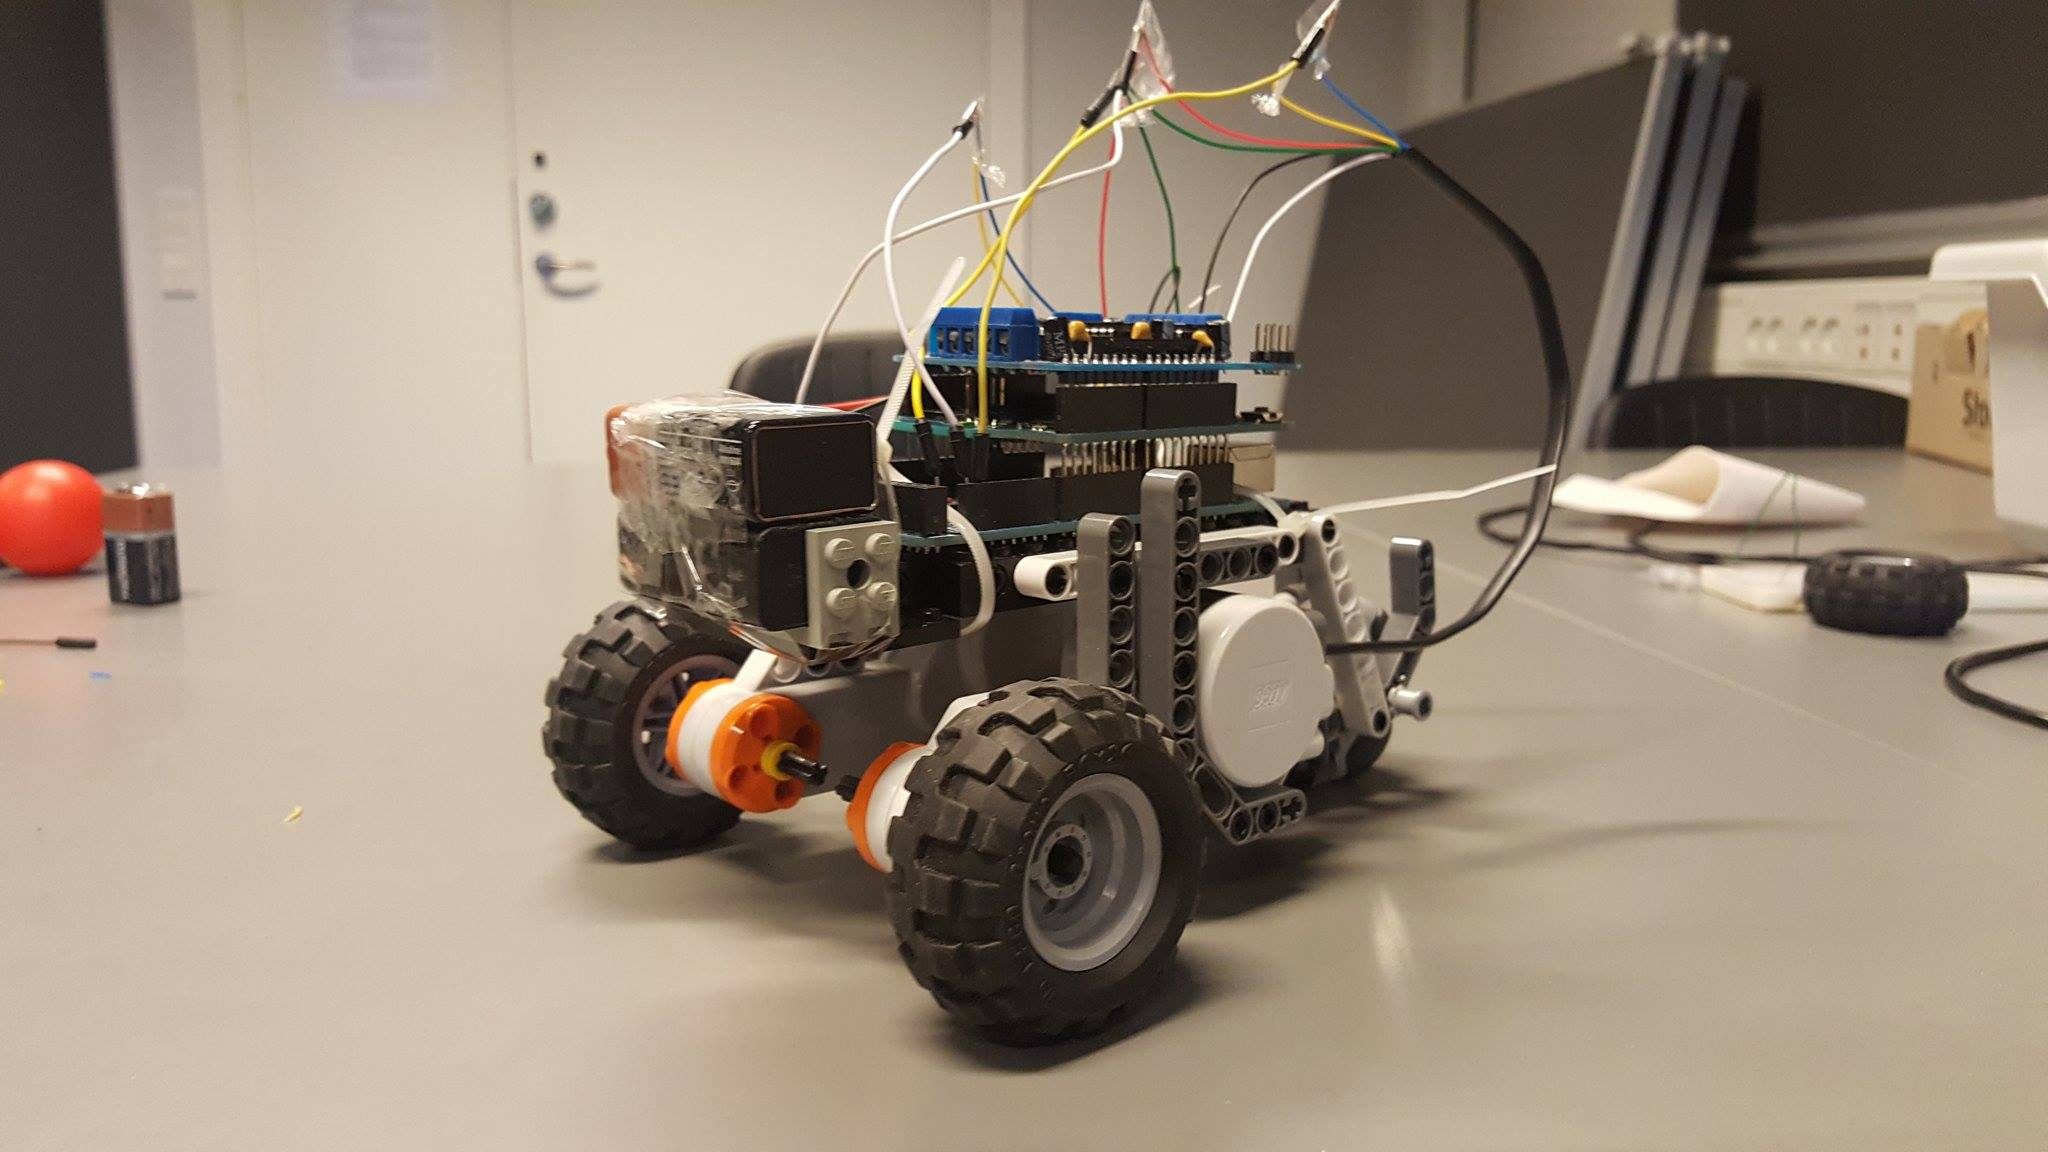
\includegraphics[scale=0.20]{billeder/robot}}
	\caption{The final design of the robot}
	\label{robot}
\end{figure}

The robot uses two LEGO NXT Servo motors with corresponding wheels, which will act as the front wheels. The back wheel can slide from side to side, which is important, since the wheel will be dragged sideways when the robots turns, whereas a normal rubber wheel would have caused a lot of friction. 
The robot is build around the NXT Servo motors, and ends with a platform at the top. The Arduino is stripped to the platform, with the shields ontop. This ensures that the Arduino does not slide off the robots platform.
The robot was build with the arduino at the top, for easy access to the different pins if needed. 

\section{Arduino program design}
\label{sec:Arduino program design}
%Dette kan indeholde hvad vores program skal kunne gøre og evt. en punktform over hvilke funktioner/tasks som programmet løber i gennem.
As mentioned in section \ref{sec:Software choices}, the arduino program was developed in the Arduino IDE version 1.0.3. The program will be responsible to move the robot to the collision point, sent by the Kinect, of the object thrown at its predefined area. This is done by the program translating the coordinates from the Kinect, into coordinates know for the robot and move to that specific location

The program have a setup and will loop the behavior of the robot. First the sets up the WiFi connection to the Kinect program, it then waits for the Kinect program to send coordinates for the impact point of the object thrown. When it have received a set of coordinates, it will then translate the coordinates to so it knows where to move to. The next steps, the arduino program will continuously loop through until the program are exited: First it will check if it is at the impact point, if it is, the program is done. Else the robot will start moving, while it keeps adjusting it direction relative to the robots heading. Finally in the loop it will update the robots current position and its heading. All this can be broken down into tasks:

\begin{itemize}
	\item Make connection to the Kinect
	\item Wait to receive coordinates from the Kinect
	\item When the coordinates are received, it will translate these to useful coordinates and then enter the behavioral loop function:
	\begin{itemize}
		\item Check if already at the collision point, if it is exit program
		\item Start moving, adjust direction relative to heading
		\item Update the its position
	\end{itemize}
\end{itemize}
 

\section{Robot positioning and movement}
\label{sec:Robot positioning and movement}
%Kan indeholde hvordan vi har tænkt os med robottens kordinatsystem og hvordan den skal bevæge sig op i mod det punkt som den får fra kinecten.
The idea for moving the robot would be to send coordinates to the robot, which would be converted to explicit millimetre values of the distance from the starting point (0, 0). This starting point delimits a predefined area, as described in \ref{sec:i1Predefined areaImplementation}, which is the area in which the robot should catch the thrown object. This area is defined by the robots capabilities and limitation. This area would allow the robot to calculate the distance travelled, and compare that value to the distance of the received coordinate. The NXT Servo motor encoders should be used to calculate the distance travelled.
If the robot has read a coordinate and started to move towards it, receiving a new coordinate would redirect the robot to the new coordinate instead. As described in \ref{sec:i1MovementImplementation}, the robots maximum speed was 25.5 cm/s, but it was significantly slower moving backwards than forwards. This resulted in the definition of the robot always starting at the coordinate (0, 0), and not considering any trash thrown behind the robot. The predefined area was determined to only be in front of the robot, to ensure that the robot does not move backwards. 

\section{Connecting Arduino and Kinect}
\label{sec:Connecting Arduino and Kinect}
%Kan indeholde hvordan vi har tænkt os at de skal kunne snakke sammen og hvilket data der skal blive sendt i mellem dem.
For convenience, and as a part of the requirements for this project, the Arduino should receive wireless data from a computer, connected to the Kinect. The Arduino Wifi Shield makes this possible, with the Wifi library included in the Arduino IDE. \newline
The connection between the Arduino and the computer should be through a local router, with a set SSID and password. The computer should use the Kinect to calculate an impact point of the object, and send this in a specific format, so that the data can be easily read and translated to a set of coordinates for the robots movement. The computer should be able to send coordinates more than once, since the first impact point is not necessarily be precise enough to catch the object. The computer should calculate increasingly accurate impact points, which should be sent with a certain minimal inter-arrival time, to not hinder the robots movement, and yet still in time for the robot to correct itself. \newline
The Arduino should receive this data and read whenever it has sufficient time to do so, and convert the data received to match the right coordinate in the predefined area. 

\section{Scheduling}
\label{sec:Scheduling}
%Snakke om de forskellige tasks, deres deadlines og hvliken metode vi vil bruge til at schedule?


\subsection{Cyclic Executive}
\label{sec:Cyclic Executive}

A cyclic executive is a model which assumes a fixed set of periodic tasks. The model is about designing an entirely static schedule in which the tasks are cyclically executed at their rate, since they are periodic, and must also meet their deadline. The model is cyclic since when the last task ends and the allotted time of a cycle ends, a new cycle begins, with all tasks placed in the same specific order as the previous cycle. The creation of such a schedule proves by construction that the tasks will always meet their deadlines at runtime, if the assumptions of the model are true. \newline
To ensure that the cyclic executive is in synchronization with real elapsed time, synchronization points are inserted into the code that implements it (maybe give an example of us doing so, or at least mention it)
Once cyclic executives are constructed, the implementation is simple and efficient since there is little overhead since there is no scheduling at runtime. Cyclic executives can be constructed separately from the system, by hand or by a tool.

-Cyclic executive “processes “ cannot be isolated from each other which can be a problem. And hard to include nonperiodic tasks.

This discussion will not feature concurrency correctness concerns with race conditions and deadlocks.

\subsection{Interrupts and their definition}
\label{sec:Interrupts and their definition}
To talk about interrupts we first need to define what we are talking about, these definitions are taken from the source. The definition for an interrupt is twofold, as the first part is as follows: “a hardware-supported asynchronous transfer of control to an interrupt vector based on the signaling of some condition external to the processor core”. The second part of the definition is: “an interrupt is the execution of an interrupt handler : code that is reachable from an interrupt vector”. The definition for the introduced term interrupt vector: “a dedicated or configurable location in memory that specifies the address to which execution should jump when an interrupt occurs”. Interrupts often but not always return control flow to where, the interrupt disrupted control flow. Interrupts often change the state of main memory, and that of device drivers, but does not disturb the main processor context of the computation which was disturbed. Missing Interrupt controller, shared interrupts, i don't think we that. \newline
A interrupt is pending when it's firing condition has occurred, the interrupt controller has been updated and the interrupt handler has not started executing. A missed interrupt is when the firing condition occurs but it does not become pending, this is usually because the interrupt is currently pending. Most hardware platforms use a bit to distinguish whether an interrupt is pending or not, a queue could perhaps be implemented through software. Hardware support can be used to disable interrupts by manipulating bits in hardware registers either through the master interrupt enable bit, or the enable bits for each interrupt. 

The following conditions decide when the firing condition for interrupt is true:

\begin{itemize}
	\item The interrupt is pending
	\item The processors master interrupt enable bit is set
	\item The enable bit for each interrupt bit is set
	\item The processor is in between executing instructions
	\item There exists no higher priority interrupt which fulfills 1-4.
\end{itemize}

Another important part of interrupts is interrupt latency, which is the time between the interrupt firing conditions become true, and the first instruction of the interrupt handler has begun executing. Nested interrupts is when an interrupt handler is preempted by another interrupt. An important distinction between threads and interrupts is that thread scheduling is through software, while interrupt scheduling is through hardware interrupt controller.


Missing subjects: Stack Overflow. Interrupt overload. Real time deadlines.
\chapter{Implementation}
\label{chap:Implementation}
This chapter will describe the implementation of the systems components. It will cover the description of the Microsoft Kinect, the robot's code and how the scheduling is done. 

\section{Microsoft Kinect}
\label{sec:Microsoft Kinect Implementation}

\section{Robot}
\label{sec:Robot}

\section{Scheduling}
\label{sec:Scheduling implementation}

\subsection{UPPAAL schedulability analysis}
\label{sec:UPPAAL schedulability}
As described in Appendix \ref{sec:i3UPPAAL model}, Dumpsty contains three tasks: PrA, PrB and PrC. These three tasks all have individual WCET, which is not calculated, but rather tested, since calculating these through assembly proved to be impossible due to unbound loops in libraries. After testing the individual task's WCET, the worst case found would be significantly faster than what is labelled in UPPAAL, since the probability of hitting the actual worst case is close to impossible with the amount of tests done. In the following bulletpoints, all three tasks tested WCET and the WCET used in UPPAAL for the specific task is expressed, which is the first step to verify the schedulability of Dumpsty's tasks.

\begin{itemize}
	\item PrA \tab Tested: 1067 microseconds \tab UPPAAL: 2 milliseconds
	\item PrB \tab Tested: 732  microseconds \tab UPPAAL: 1 milliseconds
	\item PrC \tab	Tested: 8469 microseconds \tab UPPAAL: 9 milliseconds
\end{itemize}

For convenience, and to simplify the analysis, all tasks contain the worst case runtime of all interrupts and interrupt handlers that might occur during the execution of the task. These interrupts are generated by the motor encoders when Dumpsty is moving.

Figure 5.1 depicts the automatas created in UPPAAL from two declared classes. The first class, task PrA, is the cyclic executive instance for the task PrA. The second class is simply a CPU which is the key needed to run the task. Every task can grab the CPU, but only one may hold it at any given time. The CPU is then released when the task is done executing, and another task can then proceed to run.

\begin{figure}[h]
	\centering
	\fbox{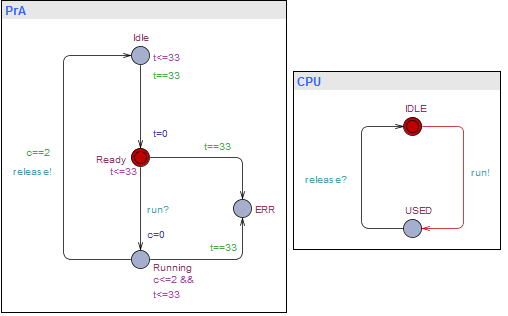
\includegraphics[scale=0.60]{billeder/UPPAALPr}}
	\caption{Automata in UPPAAL}
	\label{robot}
\end{figure}

\chapter{Tests}
\label{chap:Tests}

\section{UPPAAL schedulability analysis}
\label{sec:UPPAAL schedulability}
As described in Appendix \ref{sec:i3UPPAAL model}, Dumpsty contains three tasks: PrA, PrB and PrC. These three tasks all have individual WCET, which is not calculated, but rather tested, since calculating these through assembly proved to be impossible due to unbound loops in libraries. After testing the individual task's WCET, the worst case found would be significantly faster than what is labelled in UPPAAL, since the probability of hitting the actual worst case is close to impossible with the amount of tests done. In the following bulletpoints, all three tasks tested WCET and the WCET used in UPPAAL for the specific task is expressed, which is the first step to verify the schedulability of Dumpsty's tasks.

\begin{itemize}
	\item PrA \tab Tested: 1067 microseconds \tab UPPAAL: 2 milliseconds
	\item PrB \tab Tested: 732  microseconds \tab UPPAAL: 1 milliseconds
	\item PrC \tab	Tested: 8469 microseconds \tab UPPAAL: 9 milliseconds
\end{itemize}

For convenience, and to simplify the analysis, all tasks contain the worst case runtime of all interrupts and interrupt handlers that might occur during the execution of the task. These interrupts are generated by the motor encoders when Dumpsty is moving.

Figure \ref{UPPAAL Automata} depicts the automatas created in UPPAAL from two declared classes. The first class, task PrA, is the cyclic executive instance for the task PrA. The second class is simply a CPU which is the key needed to run the task. Every task can grab the CPU, but only one may hold it at any given time. The CPU is then released when the task is done executing, and another task can then proceed to run.

\begin{figure}[h]
	\centering
	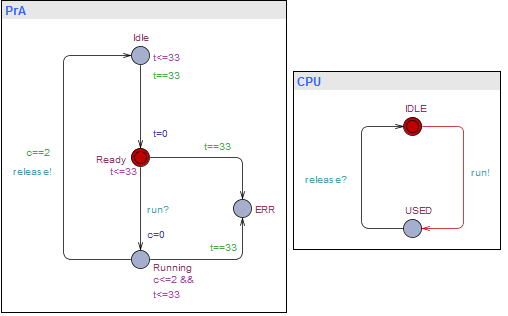
\includegraphics[scale=1]{billeder/UPPAALPr}
	\caption{Automata in UPPAAL}
	\label{UPPAAL Automata}
\end{figure}

In UPPAAL these automatas might have more than one instance, defined by the amount of tasks declared. In this case, there are three instances of the first class:

\begin{itemize}
	\item PrA = TASK(1, 33, 2);
	\item PrB = TASK(2, 33, 1);
	\item PrC = TASK(3, 33, 9);
\end{itemize}

The integers declared for every task have different meanings. These integers will be explained by the case task PrA. In task PrA, the integer 1 is the ID for the task, 33 is the deadline for the task in milliseconds, and 2 is the worst-case execution time for the task. The deadline for all tasks is the same, since this is the minimal interarrival-time(MIT) for coordinates from the Kinect sensor. All code has to be executed within the MIT of these coordinates, since a new coordinate will alter the path the robot choose.

The last step in the UPPAAL schedulability analysis is to use the verifier. This is done with two queries, found in listing \ref{Queries}. The first query checks if after some amount of time, greater than zero, all tasks has been executed at least once and all tasks are in the ready state. The second query checks that no task ever hits an error-state. If these two queries both succeed, the tasks can all be executed within the deadline, and the schedulability analysis is successful, and in this case, with tasks PrA, PrB and PrC, the tasks are schedulable within the deadlines.

\begin{lstlisting}[caption={Queries for UPPAAL}, label={Queries}]
E<> PrA.Ready and PrB.Ready and PrC.Ready and PrA.t==0 and PrB.t==0 and PrC.t==0 and time>0
E[] not (PrA.ERR or PrB.ERR or PrC.ERR)
\end{lstlisting}

\section{Unit test}
\label{sec:Unit test}
To make the unit test on the arduino code, the library ArduinoUnit has been used \citep{au}. For the arduino code there have been conducted 12 unit tests, which have been split up into two different kind of unit tests, to test the two functions driveTowardsGoal() and updatePosAndHead(). \newline
The coordinates sent to Dumpsty in the unit tests are simulated, since this is the best representation of how this robot would work under perfect conditions. These unit tests reflect how Dumpsty performs in an environment with instantaneous received data from a sensor with great precision, where the sensor will send new data every 33ms. 
The first type will test the function driveTowardsGoal() and has 3 different inputs being starting position, goal position and the heading of the robot. The robot will start at its starting position with the given heading and will then have to move towards the goal position. In the description of the test, if no heading described the heading is 0. For a code near prospective of this unit test type, check listing \ref{ut1}.

\begin{lstlisting}[caption={First type of Unit test}, label={ut1}]
test(curPos30\_150goalPos30\_150Head1){
	heading = itok(1);
	posX = itok(30);
	posY = itok(150);
	goalX = itok(30);
	goalY = itok(150);
	String result = driveTowardsGoal();
	assertEqual(result, "goal");
}
\end{lstlisting}

The second type of unit test will test the function updatePosAndHead(). The test takes 4 inputs being the starting position, the heading, millimetres to move on the right motor and millimetres to move on the left motor. The robot will start at its starting position with the given heading, and will move the given millimetres for each motor. Then the unit test will check if the robot is within 0.01mm of the asserted position.  An example of this type of unit test can been found in listing \ref{ut2}.

\begin{lstlisting}[caption={Second type of Unit test}, label={ut2}]
test(pos300_250Head075Left12Right5){
	heading = ftok(0.75);
	posX = itok(300);
	posY = itok(250);
	rightTotal = 5;
	rightTemp = 0;
	leftTotal = 12;
	leftTemp = 0;

	updatePosAndHead();

	assertMore(posX, ftok(302.826));
	assertLess(posX, ftok(302.836)); 

	assertMore(posY, ftok(253.034));
	assertLess(posY, ftok(253.044));

	assertMore(heading, ftok(0.717));
	assertLess(heading, ftok(0.727));  
}
\end{lstlisting}

Table \ref{table:Unit tests} includes all the unit tests made for the arduino code. The table consists of a description of the unit test and if the test passed or failed. 
\begin{table}
\begin{center}
	\begin{tabular}{ | p{10cm} | p{5cm} |}
		\hline
		\textbf{Test description} & \textbf{Result} \\ \hline	
		The robot is at position (30, 150), and gets the same coordinate sent, this will check if the robot says it is at goal or will try move to a new position. & Passed \\ \hline
		The robot will have a starting position at (0, 0) and will be given a new coordinate at (0, 150), the robot should then drive forward in a straight line. & \textcolor{red}{Failed} \\ \hline
		The robot will start at position (0, 0) with a heading of (1) and will be given the new coordinate (0, -150) which should make the robot turn left.  & Passed \\ \hline
		The robots starting position is (150, 150) with a heading of (-1) and is given a new coordinate at (140, 100). This means the robot will be pointing towards the top right and will have to drive down towards the right. & \textcolor{red}{Failed} \\ \hline
		The robot starts in position (150, 150) with a heading of (-1) making the robot point towards the top right. The robot is then given a new coordinate (300, 200), the robot should then turn around it self and move towards the top left & Passed \\ \hline
		The robots starting position is (0, 0) with a heading of (1), making the robot point towards the top left. The robot is given a new coordiante (0, 300). The robot will only use one motor till its heading is 0, and then drive forwards to the new coordinate  & Passed \\ \hline
		The robots starting position is (0, 0) and is given the new coordinate (-150, 300). The robot should the move towards the new position at the top right. & Passed \\ \hline
		The robot has the starting position (300, 250) with a heading of (0.75). The robot is ordered to drive 5mm with the right motor, and 12mm with the left motor and check if the new position is within a precision of 0.01mm of the asserted position. & Passed \\ \hline
		The robot has the starting position (160, 100) with a heading of (-0.4) and is to drive 14mm with the right motor and 3mm with the left motor. The robot should be within 0.01mm of the asserted position & Passed \\ \hline
		The robot is at starting position (120, 200) with a heading of (1). The robot is to drive 10mm with each motor, and be within 0.01mm of the asserted position & Passed \\ \hline
		The robot has the starting position (0, 0) and the robot is to drive 10mm with the right motor. The robot should be within 0.01mm of thte asserted position & Passed \\ \hline
		The robot has the starting position (0, 0) and the robot is to drive 10mm with the left motor. The robot should be within 0.01mm of thte asserted position & Passed \\ \hline
	\end{tabular}
	\caption{Table of conducted unit tests}
	\label{table:Unit tests}
\end{center}
\end{table}

All the failed test have been corrected and is now working as expected. 

\section{Functional test}
\label{sec:LasseSucks}
Now that the unit tests for Dumpsty are successful, the functionality of Dumpsty must be tested as well. This is done through a functional test, where Dumpsty is placed in an appropriate environment, and then the entire system will be tested. This is done through throwing a ball in front of the Kinect sensor, and having the Kinect print the sent coordinates, and having the robot moving to the point. The actual impact point of the ball will also be marked on the ground, and the distance between all three points will be measured in cm, shown in table \ref{table:FuncTest}. \newline
The three columns depicts the following:\newline
Predicted to impact: The distance from the predicted coordinate from the Kinect, to the actual impact point of the ball.\newline
Predicted to robot: The distance from the predicted coordinate to the robot, after the robot has stopped moving.\newline
Robot to impact: The distance from the robot after it has stopped moving, to the actual impact point of the ball.

\begin{table}
	\begin{center}
		\begin{tabular}{ | p{5cm} | p{5cm} | p{5cm} |}
			\hline
			\textbf{Predicted to impact} & \textbf{Predicted to robot} & \textbf{Robot to impact} \\ \hline
			23 & 11 & 34 \\ \hline
			11.5 & 6.5 & 14 \\ \hline
			19.5 & 8 & 26 \\ \hline
			19 & 10.5 & 26.5 \\ \hline
			36 & 8.5 & 43.5 \\ \hline
			48 & 11 & 56 \\ \hline
			9.5 & 11 & 21 \\ \hline
			16 & 5.5 & 11 \\ \hline
			49.5 & 11 & 48.5 \\ \hline
			13 & 11 & 19 \\ \hline
			
		\end{tabular}
		\caption{Table of conducted functional tests}
		\label{table:FuncTest}
	\end{center}
\end{table}

As one can see, Dumpsty is consistently close to 10 cm from the predicted coordinates, which could be caused by the servo motors drift after the motors has been released in the code. The fact that the prediction has a range of misprediction of 10 - 50 cm is either due to miscalculations in the Kinect code, or the Kinect having hardware issues, creating a distorted depth-picture.

%% Teknisk %%


%% Afrunding %%
\chapter{Discussion}
\label{chap:Discussion}
The discussion chapter will describe some of the choices made through the project and problems that have occurred. The problem and choices will be described and discussed, what happened and what could have been done differently. 

\subsubsection{Scheduling}
For the schedulability analysis, the WCET of the Arduino code had to be calculated. In the course, we learned that this could be done either with a language constructed timer, by counting clock cycles in the assembly code, or by using a tool. In our case, we used the tool Bound-T, without success. Our first idea was that a tool could provide WCET calculations for a piece of code, but because we were using libraries and loops which are not supported by Bound-T, it reported errors without a usable output. So our next idea was to calculate the WCET by analyzing the assembly code, but yet again the libraries proved to be a problem, since the source code of some libraries were inaccessible and contained unbounded loops. We tried counting the clock cycles, as shown in Appendix \ref{sec:i3Scheduling}. The next much coarser solution we tried was to estimate a worst-case running time for entire pieces of code, by using the timer implemented in the Arduino IDE. This is not a provable WCET estimate, since the odds of ever hitting the worst run time would be close to nonexistent in the little sample-size we provided. This lead to us almost doubling the WCET estimate in the UPPAAL model, as we already knew that the tasks were schedulable, even with a far greater WCET than what was estimated by the timer.

\subsubsection{Hardware choices}
To introduce other classical real-time concerns such as memory and execution time into this project, another platform smaller and slower than the Arduino Mega 2560 should’ve been chosen, since we only partly utilized the Arduino Mega 2560’s processor power. 

The two shields and their libraries for this project, the Arduino Motor Shield and the Arduino WiFi Shield, are helping us writing code to control the NXT servo motors and connecting to the network. When using both shields at the same time, some complications occurred. This is because the shields are using some of the same pins on the Arduino board. To work around this problem, it was decided to change the Arduino code such that it first connect to the network which will change a boolean to true and then initialize the motor shield components for use. This also means that it is not possible to continuously get new data from the Kinect, as it will send the first coordinate it captures and predicts of the thrown object. \newline

The motor shield should be used to control the motors, but an other solution to send the Kinect data to the arduino shield could be used. Either we should look for another WiFi component for the arduino, a bluetooth component or the robot should just be connected to the computer controlling the Kinect via a USB cable. 

As mentioned in chapter \ref{chap:Tests} about tests, the Kinect doesn’t reliably predict where the thrown object lands. In this project the depth sensor of the Kinect has been used, to calculate the impact point of the thrown object. Since the Kinect didn’t predict the impact point reliably, either the calculations made in the code should be revised or another way of using the Kinect should be taken into consideration. It is also possible that the Kinect didn’t function properly. 

Another important hardware issue in this project is the NXT servo motors. These motors capabilities severely limits the whole system’s capabilities. The motors set the boundaries of how far Dumpsty can move within a certain time limit paired with the circumference of the wheels. Having faster motors would also help on the response time of Dumpsty.


\subsubsection{Delimitations}
For this project we made two delimitations to the project, which can be found in section \ref{sec:Delimitations}. As mentioned, only one object will be thrown at any given time. This is an environmental delimitation, to not consider multiple objects at once. \newline
Another delimitation made was that the robot should not drive to coordinate points behind itself within the predefined area, but this is actually possible for the robot to do, also outside the predefined area. A problem we should have realized much earlier is that it is not possible for the robot to catch the object, unless it lands extremely close to the robot’s starting position, because of time spent processing, sending a signal and limitations of the motor. Another delimitations should have been made that the robot should not try to catch the object, but rather drive to the point where the object hit the ground. \newline
Instead the predefined area should not be considered and the robot should have a starting point at (0, 0), as shown in figure \ref{figure:discussion-graph} as the red dot. The robot should then be able to move to both of the blue crosses(direction of the old predefined area, but not limited to the old predefined area) and the green crosses behind the robot’s starting position. Meaning the robot only have a starting position at (0, 0), and the distance it can move on either axis is not limited, as it was with the predefined area. The robot should then drive to the predicted impact point of the object and just mark where the object had landed.


\begin{figure}[h]
	\centering
	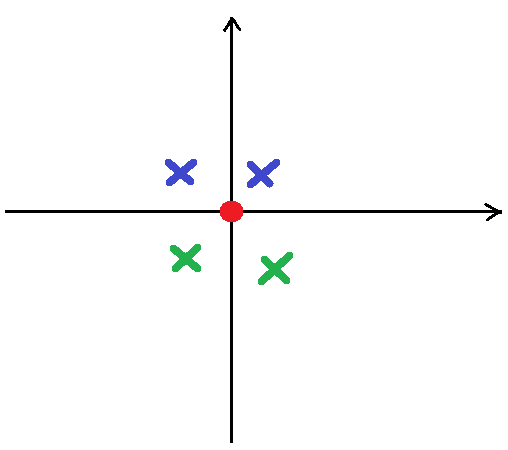
\includegraphics[scale=0.5]{billeder/discussion-graph.png}
	\caption{Graph describing the coordinate set with no predefined area}
	\label{figure:discussion-graph}
\end{figure}


\subsubsection{Process analysis}
The process model used for this project is a reflective model of the processes we have constructed our earlier projects from. This process model is based on our experience with problem based learning, and includes the processes we usually undergo through a project. It is inspired by XP, including pair programming and agile development with incrementally changing requirements. If the solution to our problem would be a safety critical solution, a more test-driven process model would be more suitable. \newline
The process model itself has worked out rather well since it isn’t restrictive and provides a very large degree of freedom when working with the project, compared to a rigid adherence to a well established model, such as the waterfall model. \newline
After experimenting with the process model throughout this project it has come to our attention that some changes should be made to the structure of the process model. A more explicit test section should be implemented to test all interdependent components, and ensure that all increments’ implementations work as intended. This will in turn also increase the coherence between each increment. This test section will also include tests across each increment, to check that no new errors has been introduced to earlier implementation.





\chapter{Conclusion}
\label{chap:Conclusion}
Based on chapter \ref{chap:Analysis} concerning a user story, system capabilities, hardware's capabilities and limitations, lead to the project’s problem statement: 


\textbf{\textit{How can an embedded system control a trash bin to detect, track and catch a thrown object within a designated area?}}


The final system partially solves the problem statement. It is capable of detecting and tracking the object thrown towards the robot, but not consistently catch it, because of the hardware limitations for the project, these limitations are mentioned in the discussion \ref{chap:Discussion}. 


To solve the problem statement, a list of general requirements with related sub requirements were constructed. In the following paragraphs each of the general requirements will be evaluated. 


\subsubsection{The trash bin should catch the object if the user throws it towards the trash bin and within a predefined area}
\label{sub:1}
This requirement was not accomplished, since the robot was not reliably able to move to the impact point of the thrown object. No trash bin has been attached on top of the robot, which would determine the area in which it is able to catch the object, but it is still considerably inaccurate by 10-50 cm from the actual impact point to the robot’s final position. If the estimated coordinate sent by the Kinect was true, it would consistently be 11 cm inaccurate, because of the robot drifting past the point after releasing the motors. \newline
We ended up not taking the predefined area into account, it was used in the design phase to measure where the robot would be able to catch a thrown object, but it was not useable because its movement was too slow and the time used in data transfer compared to object flight time was a greater obstacle than expected. Thus it was not useful in the final product.




\subsubsection{The robot should know where it is positioned}
This requirement is fulfilled. The robot has variables of its current position as an X and Y coordinate set and its heading. These values are updated in the Arduino loop function using the encoders of the motors. When the robot reaches its destination the robot shuts down, but the servo motors drift, usually 11 cm, which is not considered to the current position of the robot. This would accumulate if the robot is not reset, and placed on the position (0, 0) after every run.


\subsubsection{The robot should be able to detect and track the thrown object}
As the Kinect is used as a sensor for the robot, this requirement is fulfilled. The reason is because the Kinect is able to both detect and track the object. It is not able to detect every object thrown, and some times it detects other objects such as a human limb or something in the distortion in the room. \newline
When the first impact point of the thrown object has been sent from the Kinect, it will keep tracking the object, but the robot will not receive further data, therefore the robot is not continuously tracking the object after the first impact point is received.  


\subsubsection{The robot should be able to calculate the impact point for the object}
The Kinect sends the predicted impact point of the object to the robot. This impact point is not accurate, as mentioned before the robot is stopping 10-50 cm away from the predicted impact point. We would say that this requirement is partially fulfilled, because it can calculate an impact point, but not a precise impact point. This requirements success is scaled from how big of a bin is placed on top of the robot, and the size of the thrown object.


\subsubsection{The robot should be able to move the trash bin, such that the thrown trash lands inside the bin} 
No trash bin has been attached to the robot, so this requirement is not fulfilled. If a trash bin had been attached to the robot, it should have a radius greater than 11 cm to catch the object, since 11 cm was the closest the robot was to the impact point.


\subsubsection{The robot should be able to receive data from a computer, through a wireless network} This requirement is fulfilled. The computer connected to the Kinect is able to send the recorded data to the robot. 


\subsubsection{The system tasks should be able to be scheduled and verified}
This requirement is fulfilled by the UPPAAL schedulability analysis as described in section \ref{sec:UPPAAL schedulability} in the test chapter.


\subsubsection{Conclusion}
When considering the success of this project, the final product is somewhat a success. One can conclude that the hardware does not meet the time constraints of the problem, and the prediction is not reliable. When a user throws an object towards the robot, it is not able to catch the object, but it is able to give a prediction of the impact point, it is able to move the robot to the coordinates of the prediction, but will drift past the coordinates. The robot is able to position itself accordingly to the starting point, but it will not be able to continuously position itself after stopping at the impact point. The drift makes the robot unable to position correctly, so the robot has to be repositioned to the correct starting point after each use.\newline


The robot is able to receive data from the Kinect sensor through a wireless network, and all the tasks for the system are schedulable, and the fact that this embedded system provides a basis for a solution to the problem concludes this as a successful system in our opinion.
The biggest objective in this project was to learn about embedded systems and real time problems. Although this project did not concern many of the classical embedded systems problems, a cyclic executive was constructed and the analysis involved. Although considerations of memory management and cpu speed was not present, some considerations were performed. Even when considering the initial preconceived notions of the platform, motors and Kinect alot of unexpected problems arose, some of which were solved and others would need different hardware to solve the problem statement.  

\include{formalia/futurework}

%%%% Kilder %%%%

\begingroup
	\raggedright
	\bibliography{bibtex/litteratur}							% Litteraturlisten inkluderes
\endgroup


%%%% Fixme-listen %%%%

\newpage														% Ny side til Fixme-listen
%\listoffixmes													% Fixme-listen - fjernes til sidst i projektet med "%"


%%%% Appendiks %%%%

\appendix														% Appendiks/bilag start - giver chapter bogstaver i stedet for tal
\clearforchapter												% Sikrer at pagestylen aktiveres paa den rigtige side
\phantomsection													% Kunstigt afsnit, som hyperlinks kan 'holde fast i'
\pdfbookmark[0]{Appendiks}{appendiks}							% Tildeler en klikbar bookmark til den endelige PDF

%% Indstillinger for appendiks (deaktiveret med "%") %%

%\pagestyle{empty}												% Sidehoved/-fod for standardsider aendres til tom for appendiks
%\aliaspagestyle{chapter}{empty}								% Sidehoved/-fod for kapitelsider aendres til tom for appendiks
%\settocdepth{chapter}											% Kun kapitel-niveau vises i ToC
%\addtocontents{toc}{\protect\cftpagenumbersoff{chapter}}		% Sidetal for kapitler fjernes i ToC

%% Filer til appendiks %%

\chapter{Increment one}
\label{chap:Increment one}
In this chapter the group will go through the requirements of the project and explain how these requirements can and has been implemented. The result of this would be a new set of requirements with some of the same requirements, new requirements and changed requirements.  

\section{Requirements}
\label{sec:i1Requirements}
The requirements considered in this increment are marked with blue colouring.

\begin{itemize}
	\item When a user throws an object towards the trash bin, within the predefined area, the bin should always catch the object
	\begin{itemize}
		\item \textcolor{blue}{The robots predefined area should be calculated from the hardware limitations of the motors’ speed}
	\end{itemize}
	\item The robot should know where it is positioned
	\begin{itemize}
		\item \textcolor{blue}{The robot should have a starting position, from where it should be able to calculate it's current position }
		\item \textcolor{blue}{The robot's starting point should be placed outside its predefined area, such that it moves forward into the area}
	\end{itemize}
	\item The robot should be able to detect and track the thrown object
	\begin{itemize}
		\item \textcolor{blue}{The thrown object should be detected and tracked by a Microsoft Kinect}
		\item The Kinect should send the coordinates of the impact point of the object to the robot
	\end{itemize}
	\item The robot should be able to calculate the impact point for the object
	\begin{itemize}
		\item \textcolor{blue}{Trajectory prediction should be used to calculate the impact point of the thrown object}
	\end{itemize}
	\item The robot should be able to move the trash bin, such that the thrown object lands inside the bin
	\begin{itemize}
		\item \textcolor{blue}{The robot should be able to turn and drive forward and backwards}
		\item {The robot should be able to recognize the coordinates sent from the Kinect}
	\end{itemize}
	\item {The robot should be able to receive data from a computer, through a wireless network}
	\item {The system tasks should be able to be scheduled and verified}
\end{itemize}

These requirements are rudimentary, and the very essence of the project lies within the fulfilment of these requirements. In this increment the fundamentals of the robots movement should be implemented, the predefined area should be defined, a starting point for this area should be determined and the Microsoft Kinect should be able to detect and track an object by using trajectory prediction.

\section{System design}
\label{sec:i1System Design}
The following sections describe how the marked requirements in \ref{sec:i1Requirements} should be fulfilled. The theories and ideas will be explained subsequently.

\subsection{Predefined area}
\label{sec:i1Predefined area}
The robots predefined area, is an area where the robot should catch the object within. This area is being made because of the limitations of the robots motors and is based on motor speed and average time of a throw, so the predefined area is where the robot should be expected to catch the object within.

\subsection{Throwing}
\label{sec:i1Throwing}
The reason why the throw of the object (which in this project will be a table tennis ball) is important, is because the robot should have as much time to move to the collision point as possible. Before the robot moves to the collision point, the Kinect should calculate the where the robot should move, send the data to the robot, and the robot then moves. The Kinect can at any point send new data to the robot, so its course have to be changed, therefore it is important for the robot to have sufficient time to move within the predefined area.    

\subsection{Microsoft Kinect}
\label{sec:i1Microsoft Kinect}
To detect the object, the Kinect has to use one of its cameras, more specifically the depth sensor. The depth sensor uses a range of infrared speckles that draw a pattern in the room. Every cluster of speckles can be identified from each other, which makes the Kinect able to differentiate between objects in the room. The depth of the specific object can be determined by the use of two cameras, as both cameras can identify the speckles at the object and then triangulate the distance between the cameras and the object. This speckle pattern technology will only work indoor, and limits the use to only one kinect, as the speckles can be washed out by other lightsources.
\citep{kw}

\subsection{Trajectory prediction}
\label{sec:Trajectory prediction}
When the object, referred to in this section as the projectile, is detected and the tracking of that projectile has started, the trajectory can be predicted. This prediction is limited to the amount of data sent by the sensory camera, meaning that for every camera reading, one detection of the object is gained. The precision of the prediction will increase according to the time a projectile has been tracked. \newline 
In this project the outdoor weather conditions, that might affect the projectile trajectory, are not considered,  since the prediction is done indoor. As well, the effects of air resistance, also called drag, will not be considered.

The trajectory of a projectile is the path of a thrown projectile affected by gravity, without propulsion. To calculate a trajectory of a projectile, the initial height, the angle which the projectile is launced from, the speed of the projectile at launch and the gravitational acceleration must be taken into account. \newline 
The initial height in this project is the height at which the projectile is detected. The angle and speed at which the projectile is launched, will be calculated from the first few trackings after detecting the projectile. The gravitational acceleration is considered as \(9.81m/s^2\), which is the common value near the earths surface. \newline

To catch the projectile, the distance and time of flight have to be calculated. This is done with two mathematical formulas:
\newline 
\begin{math}
g: \ the \ gravitational \ acceleration \ (9.81m/s^2)\newline
\theta: \ the \ angle \ at \ launch 
v: \ the \ speed \ at \ launch\newline
y_{0}: \ the \ initial \ height\newline
d: \ the \ total \ horizontal \ distance \ traveled \ \newline
t: \ the \ time \ of \ flight\newline
v_{vert}: \ the \ vertical \ velocity\newline
v_{hori}: \ the \ horizontal \ velocity\newline
t_{h}: \ the \ time \ since \ first \ detection\newline
d_{t}: \ the \ distance \ at \ time \ t\newline
\end{math}

The above variables can express the formulas needed to provide the total distance traveled by the projectile, and the time of flight.\newline

Distance traveled:
\[d = \dfrac{v \ cos \ \theta}{g}(v \ sin \ \theta + \sqrt{(v \ sin \ \theta)^2 \ + \ 2gy_{0}})\] \newline
Time of flight:
\[t = \dfrac{d}{v \ cos \ \theta} = \dfrac{v \ sin \ \theta \ + \ \sqrt{(v \ sin \ \theta)^2 \ + \ 2gy_{0}}}{g}\]
\newline

To predict the trajectory of the projectile, the altitude and distance of the projectile at any time during the flight must be calculated, according to the initial height ( \(y_{0}\) ):
\[y = v_{vert}t - \dfrac{1}{2} gt^2\]
\[d_{t} = v_{hori}t\]

After this section, the projectile can be tracked, and the path for a given projectile can be calculated to a certain degree of precision. 

\subsection{Gyroscope and Accelerometer}
\label{sec:i1Gyroscope and Accelerometer}
For positioning the robot, the Lego NXT Gyro and Accelerometer sensors will be considered. These sensors will be used together to position the robot, as the gyroscope will tell the number of degrees the robot has turned, which is relative to the heading of the robot at the first recording of data. This heading will be used together with an accelerometer, which can be used to calculate the distance the robot has traveled since the first recording of data. The speed, travel time and heading will be the data of these sensors.


\subsection{Movement}
\label{sec:i1Movement}
The robot is expected to be able to drive both forward and backwards. The robot is expected to turn using either one active wheel, or using both wheels in a counterclockwise motion in order to turn faster.


\section{Implementation}
\label{sec:i1Implementation}
This section explains how the marked requirements has been implemented and whether or not the group changed the requirement, as something didn't work out as expected. 

\subsection{Gyroscope and Accelerometer in use}
\label{sec:i1Gyroscope and Accelerometer in use}
For the implementation of the gyroscope and the accelerometer, a test has to be done, to benchmark the precision of the sensors. For this, the data sent from the Arduino when the sensor has been plugged into the Arduino, was plotted in the Serial Plotter, which is a feature in the Arduino IDE. 

The accelerometer would not be precise enough to calculate the distance the robot had moved. The accelerometer would give an acceleration, to calculate from an acceleration to a distance, the time had to be multiplied to the acceleration twice. If the acceleration was not precise, this would lead to a big margin of error. 

The gyroscope worked just fine, but when it was not moving, the data seen in the Serial plotter would wander. This meant that when reading data from the gyroscope, either the gyroscope should be reset before reading data or the value would be the difference of when it started reading till it stopped. 

Instead of using the gyroscope and the accelerometer, it was decided to use the motor' encoderes, which can be used to calculate the heading and the distance moved. 


\subsection{Predefined area}
\label{sec:i1Predefined areaImplementation}
The robots predefined area will be calculated using the time of flight and the speed of the motors. 
This predefined area is limited to be strictly in front of the robot.
A bouncing throw would have a travel time of 2 - 2.15 seconds, explained in greater detail in section \ref{sec:i1ThrowingImplementation}. The predefined area was constructed using the robot itself. The robot was placed marking its starting point, and was set to turn a specific number of degrees and move forward for two seconds. After a series of runs, the area marked by the robot turned out as shown in figure \ref{figure:Predefined area}. The predefined area measures 2851.5cm\begin{math}^2\end{math}.

\begin{figure}[h]
\centering
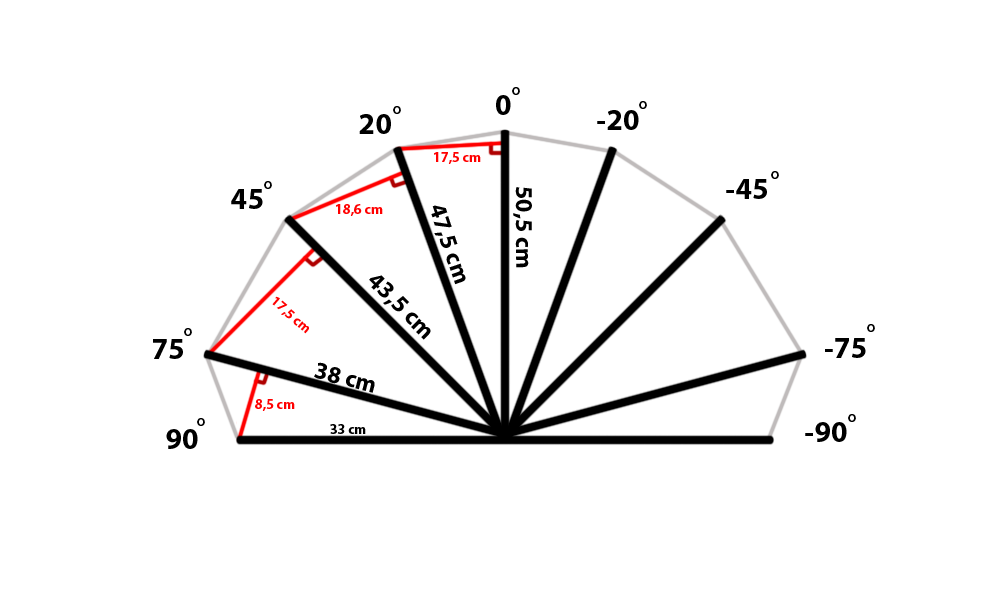
\includegraphics[scale=0.35]{billeder/predefined-area}
\caption{The robots predefined area}
\label{figure:Predefined area}
\end{figure}

\subsection{Throwing}
\label{sec:i1ThrowingImplementation} 
To ensure that the robot is provided the maximum amount of time for calculations and movement, the average time of flight of an object at a designated distance was measured. At a distance of three meters, the average time of flight of the object was 1.1 seconds, and at a distance of five meters, the average time of flight was 1.25 seconds.

With the results from the abovementioned measurements, it is concluded that a regular throw would not provide enough time for the robot to catch the object. As mentioned in the \ref{sec:LEGO NXT Servo motor} section, the robots speed was calculated to be ~87 RPM. With a 1.1 seconds time of flight, with a distance of three meters, the impact point should be within a 280 mm radius from the robot. This simply is not fast enough to catch the object from a three or five meter distance.

This introduces the idea of bouncing the object, in order to solve the above mentioned problem. The idea is, that the initial height of the object is considered to be the floor instead of the top half of the arc, which in theory should provide more time for the robot. \newline
After conducting another set of tests, this theory proved to be correct. The average time of flight at a distance of three meters is 2 seconds, and at a distance of five meters the average time of flight is on average 2.15 seconds. The bouncing throw provides the robot with close to double the amount of time.

\subsection{Microsoft Kinect}
\label{sec:i1Microsoft KinectImplementation}

\subsection{Movement}
\label{sec:i1MovementImplementation}
An Arduino Motor Shield is used to enable greater control of the movement of the motors through the motor shields library called Adafruit which is included through \#include <AFMotor.h> (unsure how to present this nicely)
The Arduino Motor Shield and library enables manipulation of the individual wheels instead of only being able to either rotate forward or backwards on both wheels simultaneously. 
The wheels were tested and forward motion was achieved with a speed of roughly 25.5 centimetres per second. It was discovered that the speed at which the robot drives backwards is much slower than its forward moving speed, because of the speed of backwards motion, it was decided to not consider driving backwards at all since the speed were inadequate and since this would also simplify the problem, and could later be solved with different motors. To solve this issue, it was decided to change the throw to always be in front of the machine, thus ensuring it would never be forced to drive backwards. This does however not take into account if the Kinect projectile prediction predicts the projectile will land behind the machine but this issue only arises if prediction is sufficiently miscalculated which is unlikely.

\section{Evaluation}
\label{sec:i1Evaluation}
This section will include a short summary of the chapter, ending up with a new requirement list, based on the how the group implemented the marked requirements from the beginning of the chapter.


The requirements stating that the robot should know where it is positioned, will persist through this increment, as no solution was found in this increment. The use of a gyroscope and accelerometer was not the right solution for this project, as the need of precise data would not be supported by sensors with a large amount of jitter. Another way of positioning the robot would be by calculating the distance traveled on each wheel, through the motor encoder in the NXT servo motors. The distance traveled would be calculated by the rotation of the wheel and the circumference of that wheel.
The robots starting position will always determine where the predefined area of the robot is along with its hardware limitations. The concept of a predefined area is entirely based on the rotation speed of each motor, the wheel circumference and the duration of the throw. If any element that defines the predefined area changes, then so does the predefined area. Movement was not nearly as simple as expected and the implications of the problems encountered in its implementation is not fully solved in this increment.

The requirement of driving forward and backwards is redefined as only consisting of driving fowards. The reason for the change was explained in the section \ref{sec:i1Movement}.

The requirements after finalizing increment one is:
\begin{itemize}
\item The trash bin should catch the trash if the user throws it towards the trash bin and within a predefined area
\begin{itemize}
	\item \textcolor{green}{The robots predefined area should be calculated from the hardware limitations of the motors’ speed}
\end{itemize}
\item The robot should know where it is positioned
\begin{itemize}
	\item \textcolor{red}{The robot should have a starting position, from where it should be able to calculate it's current position through calculations of the motor encoders}
	\item \textcolor{green}{The robot's starting point should be placed outside its predefined area, such that it moves forward into the area}
\end{itemize}
\item The robot should be able to detect and track the thrown trash
\begin{itemize}
	\item \textcolor{green}{The thrown trash should be detected and tracked by a Microsoft Kinect}
	\item The Kinect should send the coordinates of the impact point of the trash to the robot
\end{itemize}
\item The robot should know where the the thrown trash will land
\begin{itemize}
	\item \textcolor{green}{Trajectory prediction should be used to calculate impact point of the thrown trash}
\end{itemize}
\item The robot should be able to move the trash bin, such that the thrown trash lands inside the bin
\begin{itemize}
	\item \textcolor{orange}{The robot should be able to turn and drive forward}
	\item {The robot should be able to recognize the coordinates sent from the Kinect}
\end{itemize}
\item {The robot should be able to receive data from a computer, through a wireless network}
\item {The system tasks should be able to be scheduled and verified}
\end{itemize}

\chapter{Increment two}
\label{chap:Increment two}
This chapter is just like the chapter above. The results from increment one will be discussed and implemented and this should result in the same, new or changed requirements as well.  

\section{Requirements}
\label{sec:i2Requirements}
The requirement marked with blue will be considered throughout this chapter.

\begin{itemize}
	\item The trash bin should catch the trash if the user throws it towards the trash bin and within a predefined area
	\begin{itemize}
		\item {The robots predefined area should be calculated from the hardware limitations of the motors’ speed}
	\end{itemize}
	\item The robot should know where it is positioned
	\begin{itemize}
		\item \textcolor{blue}{The robot should have a starting position, from where it should be able to calculate it's current position through calculations of the motor encoders}
		\item {The robot's starting point should be placed outside its predefined area, such that it moves forward into the area}
	\end{itemize}
	\item The robot should be able to detect and track the thrown trash
	\begin{itemize}
		\item {The thrown trash should be detected and tracked by a Microsoft Kinect}
		\item \textcolor{blue}{The Kinect should send the coordinates of the impact point of the trash to the robot}
	\end{itemize}
	\item The robot should know where the the thrown trash will land
	\begin{itemize}
		\item {Trajectory prediction should be used to calculate impact point of the thrown trash}
	\end{itemize}
	\item The robot should be able to move the trash bin, such that the thrown trash lands inside the bin
	\begin{itemize}
		\item {The robot should be able to turn and drive forward}
		\item {The robot should be able to recognize the coordinates sent from the Kinect}
	\end{itemize}
	\item \textcolor{blue}{The robot should be able to receive data from a computer, through a wireless network}
\end{itemize}

\section{System design}
\label{sec:i2System design} 
In this section, the marked requirements should be fulfilled and will be described and explained.  

\subsection{Wifi Shield}
\label{sec:Wifi Shield SD}
When the Kinect have found the coordinates for the collision point of the thrown object, these coordinates should be sent to the robot, for it to be able to move to the collision point and catch the object. 
The data should be sent, as earlier mentioned in section \ref{sec: Arduino Wifi Shield}, to the Arduino wifi shield. The Arduino and the computer running the Kinect program should be connected to their own network, with the computer sending data to the wifi shields IP-address.

\subsection{Robot positioning}
\label{sec:Robot positioning System Design}
In the previous chapter, it was decided to use the motor's encoders to calculate the heading of the robot and the distance it has moved. The encoders will keep track of the number of degrees the specific motor have turned, which can be calculated to a distance using the wheels circumference.
The coordinate set for the collision point of the object and the robots current position, will be used to calculate the heading, which the robot should have to reach the collision point. 

\section{Implementation}
\label{sec:i2Implementation}
This section explains how the marked requirements were actually implemented in the project and whether or not the requirements have been changed, removed or been fulfilled. 

\subsection{Wifi Shield}
\label{sec:Wifi Shield Implementation}
To implement the Wifi Shield as part of the Arduino, the router connecting the Wifi Shield with a computer had to be port forwarded. The private network hosted by the D-link router had a specific ssid and password, which had to be explicitly assigned in the Arduino code for the Wifi Shield. The setup in the Arduino code was used to start the connection between the computer and the Wifi Shield, as well as printing the log of the connection. The setup for the wifi shield can be found in listing \ref{ws}.

\begin{lstlisting}[caption={Connecting the Wifi shield to the network}, label={ws}]
void setup() {
Serial.begin(9600);

Serial.println("Attempting to connect to WPA network...");
status = WiFi.begin(ssid, pass);

if ( status != WL_CONNECTED) { 
Serial.println("Couldn't get a wifi connection");
while(true);
} 
else {
server.begin();
Serial.println("Connected to network");
}
ip = WiFi.localIP();
Serial.println(ip);
}
\end{lstlisting}

After connecting the Wifi Shield to the router, the Arduino is ready to receive data. The data will be sent from a laptop, which connects and sends data as shown in \ref{cws}. A tcpClient is created and connected to the IP of the Wifi Shield, and the port that has been forwarded. The data sent in the code is a string "test", which is sent as a byte-array, and after sending the data, the tcpClient closes the connection.

\begin{lstlisting}[caption={Connecting the computer to the Wifi Shield}, label={cws}]
tcpClient.Connect("192.168.0.100", 9999);
string data = "test";
const int IntSize = 4;
byte[] bytedata;
Stream stream = tcpClient.GetStream();

stream.Write(Encoding.UTF8.GetBytes(data.ToCharArray()), 0, data.Length);
tcpClient.Close();
\end{lstlisting}

When both the computer and the Wifi shield has made the connection, and the computer has sent the data, the Arduino can then receive the data. This is done through a Wifi client, from the Arduino Wifi library. When assigning the client to the server.available, the value of the client in an if-statement would be true if any client from the server has data available for reading, or false if no data was available. If a client is connected, and the client has data available for reading, the next byte will be appended on the string readString, and after all the data available has been read, the full string sent by the client will be printed.

\begin{lstlisting}[caption={Receiving data from the computer}, label={rdc}]
client = server.available();
while (client.connected()){
if (client.available()) {
char c = client.read(); 
readString += c;
}
}
if(readString != ""){
Serial.println(readString);
readString = "";
}
\end{lstlisting}

\subsection{Robot positioning}
\label{sec:Robot positioning Implementation}
In the top of the Arduino program, a lot of variables were declared, which can be seen in listing \ref{declarations}. The two volatile integers leftTotal and rightTotal are used to count the number of degrees the motor have turned. leftTotal and rightTotal are volatile integers because the value of the variables can be changed by other things than the code, which in this case is the motors. \newline
motorLeftRun and motorRighRun are booleans used to check whether the motors are running or not. \newline
The variable called heading have the value of the robot's heading, which in this project will be the degrees the robot's direction is pointing away from the y-axis of its predefined area. Then robot's current position will be saved as coordinates in the variables posX and posY. \newline
Several integers are declared which will get further explanation later in the section. 
Also in the top of the program some identifiers have been defined and the necessary libraries have been included to the program.  

\begin{lstlisting}[caption={The defined and declared variables}, label={declarations}]
volatile int leftTotal = 0;
volatile int rightTotal = 0;
bool motorLeftRun = false;
bool motorRightRun = false;
double heading = 0.0, posX = 0.0, posY = 0.0;
unsigned int tid;
int leftTemp, rightTemp, goalX = 230, goalY = 330, margin = 10, loopcount = 0, signalCount = 0;
\end{lstlisting}

An arduino program is split up into a setup function and a loop function, where the code in the loop function should describe the robot's behaviour. The setup function are run once for every power up or reset of the Arduino board.
The setup function can be found in listing \ref{setup}. Two pins are setup as inputs for the arduino board and an interrupt is attached to each of them. Every time a change occurs for the input pins, which in this case is every time the motors have turned 1 degree, the functions incrementLeft and incrementRight are called accordingly. The two functions increments the counters leftTotal and rightTotal which are counting the number of degrees the motors have turned. \newline
Next up the motors are turned on. This is done by setting their speed, which here is set to the highest speed possible, and then both motors are ret to RELEASE, which will stop the motors. Also the booleans motorLeftRun and motorRightRun are set to false. \newline
At the bottom of the setup funtion, then leftTotal's and the rightTotal's values have been assigned to the temporary variables leftTemp and rightTemp.

\begin{lstlisting}[caption={The setup function}, label={setup}]'
pinMode(LEFTENCODERPIN, INPUT);
attachInterrupt(LEFTPINTOINTERRUPT, incrementLeft, CHANGE);
pinMode(RIGHTENCODERPIN, INPUT);
attachInterrupt(RIGHTPINTOINTERRUPT, incrementRight, CHANGE);

motorLeft.setSpeed(255);
motorRight.setSpeed(255);

motorLeft.run(RELEASE);
motorLeftRun = false;
motorRight.run(RELEASE);
motorRightRun = false;

leftTemp = leftTotal;
rightTemp = rightTotal;
\end{lstlisting}

When the arduino program enters the loop function, seen in listing \ref{loop}, the first thing it will do is to check the if-statement at line. This if-statement checks if the robot is at its desired position, which is the coordinate set sent from the Kinect(goalX and goalY). If the robot was at the position it will release both motors and exit the program, else it will skip this if statement and continue in the loop function. \newline
In lines 9-12 the difference of the desired coordinate and the current coordinate of the robot are calculated and assigned to the variables deltaY and deltaX. With these new variables the heading of which the robot should have to hit the desired point. The delta heading are calculated using the goalHeading and the current heading of the robot.\newline
In lines 14 - 23 the if-else statement checks if the robot is on the right heading. If the robot's heading is less than -0.1 it will release the right motor and drive forward with the left, making the robot turn right. The robot will do the same check for 0.1 and will release the left motor and drive forward on the right, making the robot turn left. If the robot is on its right heading, it will drive forward, towards it desired point. \newline
In lines 25-35 two new integers, currentLeft and currentRight, are assigned the values of leftTotal and rightTotal. Then the distance of how much the wheels have moved since last time it was looped through is calculated. This is done by taking the difference of currentLeft and leftTemp times DISTPRDEGREE, which was defined at the beginning of the program, the same is done with currentRight and tempRight. Then leftTemp and rightTemp are assigned the values of currentLeft and currentRight. \newline
The distance the robot have moved is the average of how much the two motors have moved, so the the distances of the two motors are added together and divided by two. With the distance, the robots new current position is calculated assigned to the values posX and posY, and the new heading for the robot.


\begin{lstlisting}[caption={The loop function}, label={loop}]
void loop() {
if(round(posX) <= goalX + margin && round(posX) >= goalX - margin &&     round(posY) <= goalY + margin && round(posY) >= goalY - margin){
motorLeft.run(RELEASE);
motorRight.run(RELEASE);
delay(50);
exit(0);
}

double deltaX = goalX - posX;
double deltaY = goalY - posY;
double goalHeading = atan(deltaX/deltaY);
double deltaHeading = goalHeading - heading;

if(deltaHeading < -0.1){
motorLeft.run(FORWARD);
motorRight.run(RELEASE);
}else if(deltaHeading > 0.1){
motorLeft.run(RELEASE);
motorRight.run(FORWARD);
}else{
motorLeft.run(FORWARD);
motorRight.run(FORWARD);
}

delay(10);
int currentLeft = leftTotal;
int currentRight = rightTotal;
double deltaLeft = (currentLeft - leftTemp) * DISTPRDEGREE;
double deltaRight = (currentRight - rightTemp) * DISTPRDEGREE;
leftTemp = currentLeft;
rightTemp = currentRight;
double dist = (deltaLeft + deltaRight) / 2.0;
posX += (dist * sin(heading));
posY += (dist * cos(heading));
heading += (atan((deltaRight - deltaLeft) / WHEELDIST));
}
\end{lstlisting}



\section{Evaluation}
\label{sec:i2Evaluation}
This section will include a short summary of the chapter and conclude with an updated requirement list, showing changes from the first requirement list in the chapter.
\chapter{Increment three}
\label{chap:Increment three}

\section{Requirements}
\label{sec:i3Requirements}

\begin{itemize}
	\item The trash bin should catch the trash if the user throws it towards the trash bin and within a predefined area
	\begin{itemize}
		\item {The robots predefined area should be calculated from the hardware limitations of the motors’ speed}
	\end{itemize}
	\item The robot should know where it is positioned
	\begin{itemize}
		\item {The robot should have a starting position, from where it should be able to calculate it's current position through calculations of the motor encoders}
		\item {The robot's starting point should be placed outside its predefined area, such that it moves forward into the area}
	\end{itemize}
	\item The robot should be able to detect and track the thrown trash
	\begin{itemize}
		\item {The thrown trash should be detected and tracked by a Microsoft Kinect}
		\item {The Kinect should send the coordinates of the impact point of the trash to the robot}
	\end{itemize}
	\item The robot should know where the the thrown trash will land
	\begin{itemize}
		\item {Trajectory prediction should be used to calculate impact point of the thrown trash}
	\end{itemize}
	\item The robot should be able to move the trash bin, such that the thrown trash lands inside the bin
	\begin{itemize}
		\item {The robot should be able to turn and drive forward}
		\item\textcolor{blue}{The robot should be able to recognize the coordinates sent from the Kinect}
	\end{itemize}
	\item {The robot should be able to receive data from a computer, through a wireless network}
\end{itemize}

\section{System design}
\label{sec:i3System design}

\subsection{Connecting Arduino and Kinect}
\label{sec:i3Connecting Arduino and Kinect system design}
For connecting the Arduino and Kinect, the Wifi library is used as explained in Appendix \ref{sec:Connecting Arduino and Kinect}. The Kinect should create a TCP-client, which should send the appropriate data to the Arduino. This TCP-client should connect when it can send data, and disconnect after sending the data, since the Arduino has a timer that closes the connection after 10 seconds of inactivity. The sent data should be of the form (x, z) expressing the distance from the kinect to the impact point of the object and the ground. The x-coordinate should express the horizontal position, and the z-coodinate should express the depth position. As the Kinect camera should be position and tilted so that the bottom angle of the cameras point of view is parallel to the ground, makes the y coordinate useless, as the impact point would always be at (x, (y = 0), z). This delimitation also gives the camera a sense of where the ground is, since it would not be able to see the ground, and therefore would calculate a different impact point, as the object would in a sense fall through the ground in the picture. 

\subsection{Scheduling}
\label{sec:i3Scheduling}
To be able to schedule the systems functions, the worst-case execution time(WCET) have to be known for the individual functions. The first attempt was to count the clock cycles in the assembly file of the complied arduino code. It was known that the Arduino mega 2560 has 16000 clock cycles per millisecond, so it will be possible to calculate the time for the functions. The purpose was to count the clock cycles for the two functions driveTowardsGoal and updatePosAndHead, to make that a possibility many of the functions in the different libraries used also had to be counted, the results of this can be found in Appendix \ref{chap:Clock cycles}.

In the following list, the clock cycles counted of the two functions are shown:
\begin{itemize}
	\item driveTowardsGoal = \textbf{4185} + (13)* + (174 + (13)*)* + (231 + (13)*)* + (17)* + (8)* + (33 + (17)*)* + (7)* + (5)* + (290 + (5)*)*
	\item updatePosAndHead = \textbf{3560} + (11)* + (13)* + (7)* + (174 + (13)*)* + (231 + (13)*)* (10)* + (24)* + (17)* + (33 + (17)*)*
\end{itemize}
The bold number is the worst-case of clock cycles counted in the function. The numbers in parentheses are loops, which bound is unknown, therefore it is not possible to make a count the exact WCET by counting the clock cycles.

Since it was not possible to count the clock cycles from the assembly code, it was decided to use the tool Bound-T, which will calculate the WCET outputted with an output in clock cycles. \newline
Bound-T was not able to calculate the WCET for the code. When Bound-T gets to calculating the floats, it is failing. It can't set an upper bound for the floating point numbers' WCET.

To be able to work around the float issues with Bound-T, a library called AVRFIX made by Maximilian Rosenblattl and Andreas Wolf \citep{AVRFIX}. In the listings \ref{Update1} and \ref{Update2} a function written with the AVRFIX library and a function written normally for arduino can be compared. Be aware that the function in listing \ref{Update2} might not look exactly like this in the final code for the project. 

\begin{lstlisting}[caption={The function updatePosAndHead with AWRFIX library}, label={Update1}]
void updatePosAndHead(){
	int currentLeft = leftTotal;
	int currentRight = rightTotal;
	fix_t distPrDeg = ftok(DISTPRDEGREE);
	fix_t dltL = itok(currentLeft - leftTemp);
	fix_t dltR = itok(currentRight - rightTemp);
	fix_t deltaLeft = mulk(dltL, distPrDeg);
	fix_t deltaRight = mulk(dltR, distPrDeg);
	leftTemp = currentLeft;
	rightTemp = currentRight;
	fix_t deltaSum = deltaLeft + deltaRight;
	fix_t dist = divk(deltaSum,ftok(2.0));
	fix_t sinHeading = sink(heading);
	posX += mulk(dist, sinHeading);
	fix_t cosHeading = cosk(heading);
	posY += mulk(dist, cosHeading);
	fix_t rel = divk((deltaRight - deltaLeft),ftok(WHEELDIST));
	heading += atank(rel);
}
\end{lstlisting}

\begin{lstlisting}[caption={The function updatePosAndHead from the Arduino IDE}, label={Update2}]
void updatePosAndHead(){
	int currentLeft = leftTotal;
	int currentRight = rightTotal;
	double deltaLeft = (currentLeft - leftTemp) * DISTPRDEGREE;
	double deltaRight = (currentRight - rightTemp) * DISTPRDEGREE;
	leftTemp = currentLeft;
	rightTemp = currentRight;
	double dist = (deltaLeft + deltaRight) / 2.0;
	posX += (dist * sin(heading));
	posY += (dist * cos(heading));
	heading += (atan((deltaRight - deltaLeft) / WHEELDIST));
}
\end{lstlisting}

The program was rewritten with the AVRFIX library and then using Bound-T again to calculate the worst-case execution time for the functions. The AVRFIX library came with a .txt file from the GitHub download, which included the clock cycles for the AVRFIX functions. \newline
The function updatePosAndHead is calculated to use 3995 clock cycles, but when trying to calculate the function driveTowardsGoal another problem occurred. When a division by 0 took place, the program will enter an infinite loop, making it impossible to set an upper bound on the WCET. With this problem it is not possible to calculate the WCET for driveTowardsPoint.

Because using the AVRFIX library with Bound-T also failed, the group decided to use the function micros() on the functions to measure the time spent on the function, run them several times and use highest result as WCET. 

\section{Implementation}
\label{sec:i3Implementation}

\subsection{Connecting Arduino and Kinect}
\label{sec:i3Connecting Arduino and Kinect implementation}

\section{Evaluation}
\label{sec:i3Evaluation}


\chapter{Clock cycles}
This appendix includes all the instructions from the Math.h and AFMotor.h libraries used to make the functions for the arduino program. These have all been counted by looking at the assembly code of the program. Many of the instructions have loops which is denoted with parentheses and a star, as such (7)* will be a loop of 7 clock cycles. 
\begin{itemize}
	\item \_\_fp\_Split3 = 41
	\item \_\_fp\_round = 26
	\item \_\_fp\_pscA = 11
	\item \_\_fp\_pscB = 11
	\item \_\_fp\_nan = 7
	\item \_\_fp\_inf = 10
	\item \_\_fp\_Zero = 11
	\item \_\_fp\_szero = 10
	\item \_\_addsf3x = 113 + (7)*
	\item \_\_addsf3 = 147 + (7)*
	\item \_\_fp\_cmp = 41
	\item \_\_cmpsf2 = 53
	\item \_\_subsf3 = 148 + (7)*
	\item \_\_gesf2 = 53
	\item digitalWrite = 82{\normalsize }
	\item M.latch\_tx = 572 + (290 + (5)*)*
	\item M.run = 634 + (5)* + (290 + (5)*)*
	\item delay = 52 + (6) + (51 + (6)*)*
	\item \_\_divsf3x = 229 + (17)* + (13)* + (33 + (17)*)* + (8)*
	\item \_\_divsf3 = 261 + (17)* + (13)* + (33 + (17)*)* + (8)*
	\item inverse = 269 + (17)* + (13)* + (33 + (17)*)* + (8)*
	\item interrupt = 40
	\item \_\_mulsf3x = 129 + (13)*
	\item \_\_mulsf3 = 161 + (13)*
	\item square = 163 + (13)*
	\item Powser = 130 + (174 + (13)*)* + (231 + (13)*)*
	\item atan = 989 + (13)* + (174 + (13)*)* + (231 + (13)*)* + (17)* + (8)* + (33 + (17)*)* + (7)*
	\item floatisf = 46 + (11)*
	\item \_\_fp\_splitA = 17
	\item \_\_fp\_rempio2 = 91 + (24)* + (10)*
	\item \_\_fp\_mpack = 22
	\item \_\_fp\_powsodd = 461 + (13)* + (174 + (13)*)* + (231 + (13)*)*
	\item \_\_fp\_sinus = 629 + (13)* + (174 + (13)*)* + (231 + (13)*)* + (7)*
	\item sin = 734 + (13)* + (174 + (13)*)* + (231 + (13)*)* + (7)* + (10)* + (24)*
	\item cos = 727 + (13)* + (174 + (13)*)* + (231 + (13)*)* + (17)* + (10)* + (24)*
	\item StopIfAtGoal = 979 + (7)*
	\item DriveTowardsGoal = 3206 + (13)* + (174 + (13)*)* + (231 + (13)*)* + (17)* + (8)* + (33 + (17)*)* + (7)* + (5)* + (290 + (5)*)*
	\item UpdatePosAndHead = 3560 + (11)* + (13)* + (7)* + (174 + (13)*)* + (231 + (13)*)* (10)* + (24)* + (17)* + (33 + (17)*)*
\end{itemize}
\chapter{Arduino code}
The following listing is the arduino code for this project.

\begin{lstlisting}[caption={Finished arduino code for the project}, label={ArduinoCode}]
#define LEFTENCODERPIN 20
#define RIGHTENCODERPIN 21
#define WHEELDIST 124
#define DISTPRDEGREE 0.48869219055

#include <AFMotor.h>
#include <Math.h>
#include <WiFi.h>

char ssid[] = "Dumpsty";     //  your network SSID (name) 
char pass[] = "test1234";    // your network password
int status = WL_IDLE_STATUS;     // the Wifi radio's status
IPAddress ip;
WiFiServer server(9999);
WiFiClient client;
String dataString = "";


volatile int leftTotal = 0;
volatile int rightTotal = 0;
double heading = 0.0, posX = 0.0, posY = 0.0, margin = 10.0, goalX = 0.0, goalY = 0.0;
int leftTemp, rightTemp;

void setup() {
	Serial.begin(9600);           
	status = WiFi.begin(ssid, pass);
	if ( status != WL_CONNECTED) { 
		exit(0);
	} 
	else {
		server.begin();
	}
	ip = WiFi.localIP();
	
	while(dataString == ""){
		client = server.available();
		if (client.connected()){
			while (client.available()) {
				char c = client.read(); 
				dataString += c;
			}
		}
	}
	goalX = dataString.substring(0,dataString.indexOf(';')).toInt();
	goalY = dataString.substring(dataString.indexOf(';')+1).toInt();  
	
	pinMode(LEFTENCODERPIN, INPUT);
	attachInterrupt(3, incrementLeft, CHANGE);
	pinMode(RIGHTENCODERPIN, INPUT);
	attachInterrupt(2, incrementRight, CHANGE);
	
	leftTemp = leftTotal;
	rightTemp = rightTotal;
}

void loop() {
	driveTowardsGoal();  
	delay(10);
	updatePosAndHead();
}

void updatePosAndHead(){
	int currentLeft = leftTotal;
	int currentRight = rightTotal;
	double deltaLeft = (currentLeft - leftTemp) * DISTPRDEGREE;
	double deltaRight = (currentRight - rightTemp) * DISTPRDEGREE;
	leftTemp = currentLeft;
	rightTemp = currentRight;
	double dist = (deltaLeft + deltaRight) / 2.0;
	posX += (dist * sin(heading));
	posY += (dist * cos(heading));
	heading += (atan((deltaRight - deltaLeft) / WHEELDIST));
}

void driveTowardsGoal(){
	AF_DCMotor motorLeft(1);
	AF_DCMotor motorRight(2);
	
	motorLeft.setSpeed(255);
	motorRight.setSpeed(255);
	
	if(posX <= goalX + margin && posX >= goalX - margin && posY <= goalY + margin && posY >= goalY - margin){
		motorLeft.run(RELEASE);
		motorRight.run(RELEASE);
		delay(50);
		exit(0);
	} else {
		double deltaX = goalX - posX;
		double deltaY = goalY - posY;
		double actualGoalHeading;
		if(deltaX == 0 && deltaY > 0)
			actualGoalHeading = 0;
		else if(deltaX == 0 && deltaY < 0)
			actualGoalHeading = PI;
		else
			actualGoalHeading = deltaX >= 0 ? atan(deltaY/deltaX) - (PI/2) : atan(deltaY/deltaX) + (PI/2);
	
		double deltaHeading = actualGoalHeading - heading;
		if(deltaHeading > PI)
			deltaHeading -= 2*PI;
		else if(deltaHeading < -PI)
			deltaHeading += 2*PI;
		if(deltaHeading < -0.1){
			motorLeft.run(FORWARD);
			motorRight.run(RELEASE);
		}else if(deltaHeading > 0.1){
			motorLeft.run(RELEASE);
			motorRight.run(FORWARD);
		}else{
			motorLeft.run(FORWARD);
			motorRight.run(FORWARD);
		}
	}
}

void incrementLeft(){
	leftTotal++;
}

void incrementRight(){
	rightTotal++;
}

\end{lstlisting}


%%%% Bilag %%%%

%\phantomsection												% Kunstigt afsnit, som hyperlinks kan 'holde fast i'
%\addcontentsline{toc}{chapter}{Bilag A \ Navn} 				% Manuelle indgange i indholdsfortegnelsen (naar \includepdf bruges)

%\includepdf[pages={x-y}]{filnavn}								% Inkluder eksterne bilag med \includepdf[pages={x-y}]{filnavn}


\end{document}													% Slutter dokumentet - obligatorisk


